% ============================================================
% IEEE-style report
% Compile with pdfLaTeX (IEEEtran conference)
% ============================================================
\documentclass[10pt,conference]{IEEEtran}

\usepackage[utf8]{inputenc}
\usepackage[T5]{fontenc}
\usepackage[vietnamese,english]{babel}
% VnTeX provides a complete Type-1 Vietnamese Computer Modern family.
% Use it instead of IEEEtran's Times default so portable pdfLaTeX can embed it.
\renewcommand{\rmdefault}{cmr}
\pdfmapfile{+K:/scale/.tools/ctan/vntex-tds/fonts/map/dvips/vntex/vnrtext.map}
\pdfmapfile{+K:/scale/.tools/ctan/vntex-tds/fonts/map/dvips/vntex/vnrother.map}
\pdfmapfile{+K:/scale/.tools/ctan/vntex-tds/fonts/map/dvips/vntex/urwvn.map}
\pdfmapfile{+K:/scale/.tools/ctan/vntex-tds/fonts/map/dvips/vntex/chartervn.map}
\pdfmapfile{+K:/scale/.tools/ctan/vntex-tds/fonts/map/dvips/vntex/arevvn.map}
\pdfmapfile{+K:/scale/.tools/ctan/vntex-tds/fonts/map/dvips/vntex/cmbrightvn.map}
\pdfmapfile{+K:/scale/.tools/ctan/vntex-tds/fonts/map/dvips/vntex/concretevn.map}
\pdfmapfile{+K:/scale/.tools/ctan/vntex-tds/fonts/map/dvips/vntex/grotesqvn.map}
\pdfmapfile{+K:/scale/.tools/ctan/vntex-tds/fonts/map/dvips/vntex/txttvn.map}
\pdfmapfile{+K:/scale/.tools/ctan/vntex-tds/fonts/map/dvips/vntex/vntopia.map}
\usepackage{amsmath,amssymb,amsfonts}
\usepackage{booktabs}
\usepackage{array}
\usepackage{multirow}
\usepackage{graphicx}
\usepackage{url}
\usepackage{cite}
\usepackage{enumitem}
\usepackage{balance}
\usepackage{placeins}
\usepackage{float}

% Cấu hình đánh số trang
\pagestyle{plain}

\newcolumntype{L}[1]{>{\raggedright\arraybackslash}p{#1}}

\title{Tìm kiếm hình ảnh sản phẩm đa phương thức\\
trong Thương mại Điện tử với SCALE\\
Faiss HNSW và tái xếp hạng thuộc tính}

\author{
  \IEEEauthorblockN{GVHD: TS. Võ Hoài Việt\\
                    ThS. Phạm Minh Hoàng\\
                    ThS. Phạm Thanh Tùng}
  \IEEEauthorblockA{
    Trường Đại học Khoa học Tự nhiên\\
    \phantom{MSSV: 00000000} % Giữ khoảng trống căn hàng đẹp
  }
  \and
  \IEEEauthorblockN{Sinh viên: Trần Hải Đức}
  \IEEEauthorblockA{
    MSSV: 23127173\\
    Trường Đại học Khoa học Tự nhiên\\
    thduc23@clc.fitus.edu.vn
  }
  \and
  \IEEEauthorblockN{Sinh viên: Trần Hoàng Nam}
  \IEEEauthorblockA{
    MSSV: 23127232\\
    Trường Đại học Khoa học Tự nhiên\\
    thnam23@clc.fitus.edu.vn
  }
}
\begin{document}
\maketitle
\thispagestyle{plain} % Hiển thị số trang cho trang đầu tiên

\begin{abstract}
Tìm kiếm sản phẩm thương mại điện tử trong thực tế không chỉ dựa trên ảnh mà còn khai thác tên và mô tả sản phẩm, bảng thuộc tính, video và audio. Báo cáo này nghiên cứu bài toán truy hồi sản phẩm đa phương thức trên M5Product, trong đó mỗi listing có thể thiếu một hoặc nhiều modality. Mục tiêu là trả về các sản phẩm vừa tương đồng về biểu hiện thị giác, vừa phù hợp với ngữ nghĩa thương mại và thuộc tính quyết định mua, chẳng hạn siêu danh mục, danh mục, thương hiệu và thông số kỹ thuật.

Phương pháp sử dụng SCALE (Self-harmonized ContrAstive Learning) để học unified embedding từ năm modality gồm image, text, table, video và audio. Các encoder riêng, Joint Co-Transformer, masked multimodal learning và SIMCL được dùng để mô hình hóa tương tác giữa các modality, đồng thời giảm ảnh hưởng của dữ liệu thiếu hoặc nhiễu. Trên không gian embedding đã chuẩn hóa, báo cáo đề xuất sử dụng Faiss HNSW để thu hẹp catalog thành tập ứng viên, sau đó tái xếp hạng theo metadata nhằm điều chỉnh thứ hạng cuối cùng.

Kết quả được tách thành hai nhóm metric. Với representation-only protocol tái lập nội bộ, TPIVA đạt mAP@10 0.45\%; với pipeline serving HNSW Top-100 và reranking title/PV, mAP@10 đạt 12.54\% và Precision@10 đạt 2.63\%. Báo cáo tách bạch hai nhóm này với số liệu tham chiếu SCALE, đồng thời nêu rõ chúng không phải các benchmark đồng nhất.
\end{abstract}

\begin{IEEEkeywords}
\raggedright
visual product search, multimodal retrieval, M5Product, SCALE, SIMCL,
Joint Co-Transformer, Faiss HNSW, reranking, e-commerce
\end{IEEEkeywords}

% ============================================================
\section{Giới thiệu}
% ============================================================

\subsection{Bối cảnh và Lý do chọn đề tài}

E-commerce đang chuyển từ tìm kiếm dựa hoàn toàn trên từ khóa sang trải nghiệm giàu ngữ cảnh hơn. Tìm kiếm truyền thống yêu cầu người dùng mô tả sản phẩm bằng text như tên mặt hàng, màu sắc, kiểu dáng, vật liệu hoặc thương hiệu. Cách tiếp cận này gặp khó khăn khi người dùng chỉ có ảnh hoặc video tham khảo, không biết tên chính xác của sản phẩm, hoặc khi mô tả của người bán không đồng nhất. Visual search giảm ma sát bằng cách cho phép người dùng cung cấp ảnh hoặc video, từ đó hệ thống học đặc trưng và truy hồi các sản phẩm tương tự~\cite{venkatesan2025}.

Tuy nhiên, một listing thực tế hiếm khi chỉ gồm ảnh. Sản phẩm thường có caption, bảng thuộc tính, video giới thiệu và audio tách từ video. Vì vậy, bài toán trong nghiên cứu này được mở rộng từ image-to-image retrieval sang \emph{multimodal product retrieval}: biểu diễn query và sản phẩm từ mọi modality khả dụng rồi tìm các product entry có embedding gần nhất.

\subsection{Phạm vi bài toán}

Query được biểu diễn bởi
\begin{equation}
q=(I,T,Tab,V,A),
\end{equation}
trong đó $I$, $T$, $Tab$, $V$ và $A$ lần lượt là image, text, table, video và audio. Query phải có ít nhất image hoặc video; các modality còn lại có thể thiếu. Catalog được định nghĩa là
\begin{equation}
G=\{p_1,p_2,\ldots,p_N\},
\end{equation}
với mỗi $p_i$ cũng có thể thiếu một số modality.

Mục tiêu là trả về $K$ sản phẩm trong catalog có embedding đa phương thức gần query nhất. Khác với image retrieval thuần túy, kết quả không chỉ cần giống về màu sắc hoặc texture mà còn cần phù hợp về ngữ nghĩa thương mại như siêu danh mục, danh mục, thương hiệu và các thuộc tính quyết định mua.

\subsection{Khoảng trống nghiên cứu và Đóng góp}

Các hệ thống visual product search hiện có thường tập trung vào image-only hoặc image+text. M5Product/SCALE mở rộng lên năm modality và hỗ trợ missing modality, nhưng retrieval gốc của SCALE sử dụng exact similarity giữa query và gallery, chưa giải quyết trực tiếp bài toán serving trên catalog động và chưa có tầng metadata reranking.

Các đóng góp chính của đề tài gồm:
\begin{enumerate}[leftmargin=*]
    \item Xây dựng pipeline multimodal product retrieval sử dụng SCALE để tạo unified embedding từ image, text, table, video và audio.
    \item Xây dựng lớp serving bằng Faiss HNSW để lọc nhanh $N>K$ ứng viên trên catalog và hỗ trợ thêm listing mà không cần huấn luyện lại index.
    \item Triển khai tầng reranking không dùng nhãn: trộn điểm embedding với độ tương đồng TF--IDF character n-gram trên title và PV attributes sau bước lọc HNSW.
\end{enumerate}

% ============================================================
\section{Đặc điểm sản phẩm thương mại điện tử và Dataset}
% ============================================================

\subsection{Khái niệm}
Một mẫu sản phẩm thương mại điện tử không chỉ đơn thuần là một ảnh đại diện. Trên trang listing, người mua thường thấy đồng thời hình ảnh, tên/mô tả, bảng thuộc tính, và đôi khi có cả video hay audio đi kèm. Các tín hiệu này cùng mô tả một SKU nhưng không trùng lặp nội dung: ảnh thể hiện hình dáng và màu sắc, bảng thuộc tính chi tiết về thương hiệu/chất liệu/kích thước, còn video/audio thể hiện hướng dẫn sử dụng và góc nhìn thực tế.

Trong bài toán truy hồi, mẫu sản phẩm là đơn vị retrieval cơ bản: hệ thống thực hiện so khớp biểu diễn đa phương thức của query với biểu diễn đa phương thức của từng $p_i$ trong kho catalog, thay vì chỉ so sánh từng ảnh đơn lẻ như các hệ thống image retrieval thuần túy.

\subsection{Ba tính chất then chốt}
\subsubsection{Dữ liệu có cấu trúc}
Một mẫu sản phẩm thông thường bao gồm năm thành phần modality:
\begin{itemize}[leftmargin=*]
    \item \textbf{Ảnh (Image):} Thể hiện ngoại quan (appearance), màu sắc, hình dáng sản phẩm.
    \item \textbf{Văn bản (Text):} Tên sản phẩm, mô tả chi tiết, caption, các điểm bán hàng nổi bật (selling points).
    \item \textbf{Bảng (Table):} Các cặp key-value lưu trữ thông số kỹ thuật như thương hiệu, chất liệu, kích thước, xuất xứ.
    \item \textbf{Video:} Cung cấp chuyển động đa góc nhìn, độ đàn hồi, trải nghiệm trực quan cách sử dụng.
    \item \textbf{Âm thanh (Audio):} Lời thuyết minh giới thiệu hoặc âm thanh gốc trích xuất từ video.
\end{itemize}
\textit{Ví dụ:} Xét mẫu đồng hồ Casio, ảnh mặt đồng hồ đi kèm caption dòng \texttt{Accent Color EF-130D-1A2} và bảng thuộc tính (thương hiệu, khả năng chống nước 100m, độ dày 13mm, xuất xứ Nhật Bản, loại hiển thị kim). Không một modality đơn lẻ nào có thể tự cung cấp đầy đủ thông tin để định danh sản phẩm.

\subsubsection{Dữ liệu không toàn vẹn}
Không phải listing nào trên sàn e-commerce cũng cung cấp đủ năm modality. Người bán có thể chỉ đăng tải ảnh và title, thiếu hoàn toàn bảng thuộc tính, video hay audio. Bộ dữ liệu M5Product phản ánh chính xác thực tế này: nhiều mẫu sản phẩm bị thiếu một hoặc nhiều modality, trong đó khoảng 5\% là mẫu đơn phương thức (unimodal). Hệ thống retrieval không được phép loại bỏ các mẫu thiếu này ra khỏi quá trình huấn luyện hay catalog; việc loại bỏ sẽ làm tổn thất dữ liệu và khiến mô hình kém khả năng nhúng (embedding) các listing thực tế thiếu thông tin.

\subsubsection{Dữ liệu cực kỳ đa dạng}
Catalog thương mại điện tử không giới hạn ở một ngành hàng cố định mà trải rộng từ giày dép, đồ gia dụng, nội thất, thực phẩm đến đồng hồ, balo. Hình dáng tổng thể giữa nhiều SKU có thể rất tương đồng (ví dụ: cùng kiểu dáng đế/mũi/dây giày), nhưng điểm khác biệt lại nằm ở model, màu sắc hay chất liệu. Bối cảnh chụp (background) cũng không đồng nhất: từ nền studio trắng tiêu chuẩn đến nền màu phức tạp hoặc môi trường sử dụng thực tế.

\subsection{Bộ dữ liệu M5Product}

M5Product là bộ dữ liệu đa phương thức dành cho sản phẩm thương mại điện tử, gồm 6,313,067 mẫu, 6,232 danh mục và hơn 5,000 thuộc tính~\cite{dong2022m5product}. Mỗi mẫu có thể chứa category, image, caption, table, video và audio. Hình~\ref{fig:m5product} minh họa năm modality và cách chúng cùng mô tả một sản phẩm: ảnh thể hiện ngoại quan, caption cung cấp mô tả tự do, table lưu thuộc tính cấu trúc, video ghi nhận nhiều khung hình, còn audio bổ sung tín hiệu âm thanh.

\begin{figure}[t]
\centering
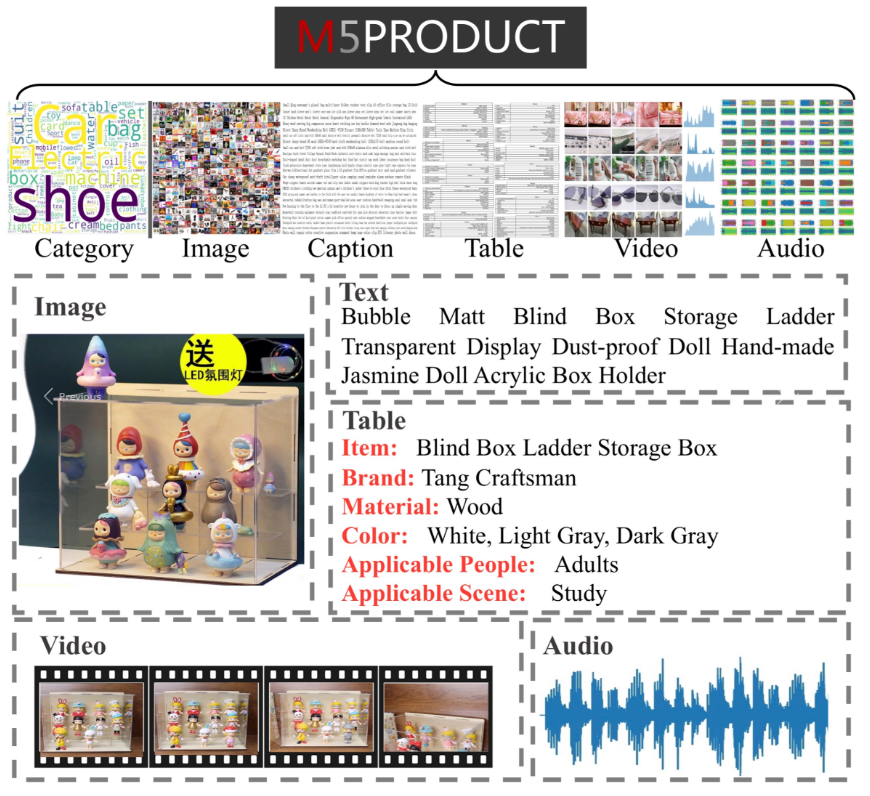
\includegraphics[width=\columnwidth]{figure/m5product.png}
\caption{Cấu trúc một mẫu trong M5Product với năm modality: image, text/caption, table, video và audio.}
\label{fig:m5product}
\end{figure}

\subsection{Xây dựng tập con 10,000 mẫu}

Do toàn bộ M5Product có quy mô lớn, nghiên cứu xây dựng một tập con 10,000 mẫu có phân bố ngành hàng và mức độ đầy đủ modality được kiểm soát. Trước hết, taxonomy được dùng để chọn 50 siêu danh mục; từ mỗi siêu danh mục lấy tối đa 200 listing hợp lệ, ưu tiên ảnh có thể đọc được và giảm trùng lặp nguồn. Sau đó, các mẫu được phân tầng theo mức độ đầy đủ modality: 7,000 mẫu có đủ năm modality, 2,000 mẫu thiếu một hoặc nhiều modality và 1,000 mẫu đơn phương thức. Việc giữ lại cả hai nhóm thiếu dữ liệu giúp đánh giá đúng khả năng xử lý missing modality thay vì chỉ đo trên listing hoàn chỉnh.

\begin{table}[t]
\centering
\caption{Thiết kế tập con M5Product dùng trong nghiên cứu}
\label{tab:subset-10k}
\small
\begin{tabular}{lrr}
\toprule
\textbf{Nhóm mẫu} & \textbf{Số lượng} & \textbf{Tỷ lệ}\\
\midrule
Đủ năm modality & 7,000 & 70\%\\
Thiếu modality & 2,000 & 20\%\\
Đơn phương thức & 1,000 & 10\%\\
\midrule
Tổng & 10,000 & 100\%\\
\bottomrule
\end{tabular}
\end{table}

\subsection{Hệ quả đối với hệ thống Retrieval}

\begin{table}[htbp]
\centering
\caption{Hệ quả kỹ thuật của các đặc điểm sản phẩm lên hệ thống Retrieval}
\label{tab:dieu_kien_retrieval}
\small
\begin{tabular}{L{2.5cm}L{5.0cm}}
\toprule
\textbf{Tính chất sản phẩm} & \textbf{Hệ quả kỹ thuật trong Retrieval} \\
\midrule
\textbf{Có cấu trúc, đa phương thức} & Bắt buộc phải có cơ chế dung hợp (fusion), do mỗi nhánh thông tin chỉ chứa một phần ngữ nghĩa của sản phẩm. \\
\midrule
\textbf{Dữ liệu không toàn vẹn} & Cần cơ chế mã hóa linh hoạt các mẫu thiếu modality (như Zero Imputation), không được bỏ qua hay xóa dữ liệu. \\
\midrule
\textbf{Đa dạng ngành hàng} & Biểu diễn không gian nhúng (embedding) phải mang tính tổng quát, không bị bó hẹp hay thiên lệch vào một ngành hàng cụ thể. \\
\bottomrule
\end{tabular}
\end{table}

Quy trình truy hồi tổng quát bao gồm: Nhận query đa phương thức $\rightarrow$ Tiền xử lý từng modality $\rightarrow$ Trích xuất không gian nhúng $\rightarrow$ So khớp trên tập catalog $\rightarrow$ Xếp hạng Top-K.

\subsection{Kết luận chuyển tiếp}
Tìm kiếm sản phẩm (Product Search) trong thương mại điện tử không phải là bài toán Image Retrieval thuần túy. Cả bộ dữ liệu lẫn phương pháp xử lý phải sát với dữ liệu thực tế: hỗ trợ đa phương thức, chịu được sự thiếu hụt modality và bao phủ nhiều ngành hàng. Đây chính là lý do nghiên cứu lựa chọn bộ dữ liệu M5Product cùng mô hình SCALE, đồng thời xây dựng tập subset 10.000 mẫu đại diện nhưng vẫn giữ nguyên tỉ lệ phân bố đầy đủ/thiếu hụt của các modality.

% ============================================================
\section{Nghiên cứu liên quan}
% ============================================================

\subsection{M5Product và SCALE}

M5Product được đề xuất để giải quyết giới hạn của pretraining đa phương thức chỉ dựa trên image--text. Dataset gồm 6,313,067 mẫu, 6,232 category, hơn 5.000 thuộc tính và năm modality: image, text, table, video và audio~\cite{dong2022m5product}. Khoảng 20\% mẫu thiếu một hoặc nhiều modality và khoảng 5\% là unimodal, phản ánh dữ liệu listing không hoàn chỉnh trong e-commerce.

SCALE sử dụng kiến trúc single-stream: mỗi modality được mã hóa bởi encoder tương ứng, token của các nhánh được kết hợp và đưa vào Joint Co-Transformer. Bên cạnh masked tasks, SIMCL học trọng số tương tác giữa các modality thay vì giả định mọi cặp modality có mức bổ trợ như nhau.

\subsection{Visual Product Retrieval}

Shopsy tập trung vào image-to-image retrieval trong điều kiện ảnh bị nén, crop, scribble hoặc logo reseller. Phương pháp kết hợp attribute classification, triplet ranking và cơ chế chống nhiễu ảnh, sau đó sử dụng ANN retrieval như HNSW/ScaNN~\cite{nadkarni2022shopsy}.

MIEM là hệ thống multimodal item embedding cho Shopee, kết hợp nhiều ảnh sản phẩm với title bằng merge-attention và xây dựng HNSW index~\cite{liu2024miem}. Tuy nhiên, query chủ yếu là ảnh và catalog không bao phủ table, video và audio.

MRSE sử dụng two-tower architecture và mixture-of-experts cho text, image và user history trong hệ thống tìm kiếm quy mô lớn~\cite{jiang2024mrse}. Hệ thống phù hợp với production search nhưng khác với bài toán năm modality của M5Product.

FashionMV/ProCIR giải quyết composed image retrieval trong miền thời trang bằng multi-view image và modification text~\cite{yuan2026fashionmv}. Phương pháp xử lý view incompleteness tốt nhưng phạm vi vẫn hẹp hơn catalog e-commerce đa ngành và năm modality.

\subsection{Điểm đặc biệt của SCALE + Faiss}

\begin{table}[t]
\centering
\caption{So sánh các hướng tiếp cận liên quan}
\label{tab:related}
\small
\begin{tabular}{L{1.65cm}L{1.65cm}L{1.1cm}L{1.15cm}}
\toprule
\textbf{Phương pháp} & \textbf{Modality} & \textbf{Thiếu Modality} & \textbf{Chỉ mục}\\
\midrule
Shopsy & Image & Không & HNSW/\allowbreak ScaNN\\
MIEM & Image + Text & Hạn chế & HNSW\\
MRSE & Text + Image + History & Không & HNSW\\
FashionMV & Multi-view + Text & Theo view & Product embedding\\
SCALE + HNSW (hiện thực) & I/T/Tab/V/A & Có & HNSW\\
\bottomrule
\end{tabular}
\end{table}

Điểm đặc biệt của hệ thống là kết hợp hai thành phần có vai trò tách bạch. SCALE là representation backbone: thay vì chủ yếu ghép image với text, mô hình học biểu diễn chung cho image, text, table, video và audio. Joint Co-Transformer cho phép các modality tương tác trực tiếp; SIMCL tự học mức độ bổ trợ giữa các cặp modality; còn zero imputation kết hợp attention mask giúp xử lý listing thiếu thông tin. Nhờ đó, SCALE học được liệu sản phẩm và query có cùng ngữ nghĩa hay không, kể cả khi dữ liệu không đầy đủ.

Faiss HNSW là lớp serving trên không gian embedding của SCALE. Sau khi SCALE tạo vector biểu diễn, HNSW tìm nhanh các ứng viên gần nhất trên catalog lớn, còn tầng metadata reranking điều chỉnh thứ hạng dựa trên thuộc tính. Sự phân tách này giúp đánh giá rõ chất lượng representation của SCALE và hiệu năng truy hồi của chỉ mục, đồng thời phù hợp hơn với bài toán product retrieval đa ngành hàng so với các hướng chỉ tối ưu image-only hoặc image--text.

% ============================================================
\section{Phát biểu bài toán (Problem Statement)}
% ============================================================

\subsection{Mục tiêu}
Giải quyết bài toán \textbf{Multimodal Retrieval} trên tập sản phẩm thương mại điện tử. Cho trước một truy vấn $q$ chứa các modality khả dụng và một kho sản phẩm catalog $G$, hệ thống cần trả về tập hợp Top-K sản phẩm có biểu diễn vector đa phương thức tương đồng nhất. Mặc dù từng listing có thể bị thiếu hụt một số nhánh thông tin, không gian nhúng được học vẫn phải bảo đảm tính nhất quán để so sánh.

\subsection{Đầu vào và Đầu ra (Input / Output)}
\begin{enumerate}[leftmargin=*]
    \item \textbf{Đầu vào (Input):}
    \begin{itemize}
        \item \textbf{Query:} $q = (\text{Image}, \text{Text}, \text{Table}, \text{Video}, \text{Audio})$. 
        Trong đó, Table là bảng thuộc tính cặp key-value; Audio được trích xuất từ Video. Theo phương pháp gốc, audio được biểu diễn bằng MFCC; pipeline hiện tại tạo log mel-spectrogram, do đó hai cấu hình này được tách riêng khi báo cáo thực nghiệm. Query chứa các modality khả dụng, trong đó \textbf{bắt buộc phải có tối thiểu Image hoặc Video}, các nhánh còn lại có thể khuyết thiếu.
        \item \textbf{Kho sản phẩm (Catalog):} $G = \{p_1, p_2, \dots, p_N\}$, trong đó mỗi $p_i = (\text{Image}_i, \text{Text}_i, \text{Table}_i, \text{Video}_i, \text{Audio}_i)$ cũng có thể không đầy đủ các modality.
    \end{itemize}
    \item \textbf{Đầu ra (Output):}
    \begin{itemize}
        \item Tập hợp $K$ sản phẩm hàng đầu $\{p_1, p_2, \dots, p_K\}$ trích xuất từ catalog $G$, đi kèm ảnh đại diện, metadata và điểm số tương đồng $\text{sim}(f(q), f(p_i))$ phục vụ hiển thị giao diện và bước tái xếp hạng.
    \end{itemize}
\end{enumerate}

\subsection{Biểu diễn toán học (Formalization)}
Ký hiệu $f(\cdot)$ là hàm mã hóa đa phương thức SCALE (bao gồm các encoder riêng biệt cho từng nhánh, cơ chế Zero-Imputation xử lý nhánh thiếu, mạng Joint Co-Transformer và lớp gom tụ Pooling).

Hàm tính độ tương đồng $\text{sim}(\cdot, \cdot)$ được định nghĩa bằng tích vô hướng giữa hai vector đã qua chuẩn hóa $L_2$ (tương đương với điểm Cosine Similarity):

\begin{equation}
\text{TopK}(q, G) = \arg \max_{p_i \in G}^K \text{sim}(f(q), f(p_i))
\end{equation}

Sau quá trình truy hồi thô bằng chỉ mục Faiss HNSW, điểm số tương đồng $\text{sim}$ này sẽ kết hợp với điểm tương đồng thuộc tính $S_{\text{thuoc\_tinh}}$ trước khi cắt ngưỡng lấy Top-K danh sách cuối cùng.

\subsection{Yêu cầu hệ thống}
\begin{itemize}[leftmargin=*]
    \item Học được không gian nhúng giàu ngữ nghĩa từ 5 modality và tự động cân bằng mức độ đóng góp của từng nhánh thông qua cơ chế SIMCL.
    \item Có khả năng mã hóa các query hoặc catalog mục thiếu modality mà không gây lỗi chương trình hay lệch phân bố vector (thông qua cơ chế Zero Imputation).
    \item Khả năng truy hồi thời gian thực trên catalog quy mô lớn; hỗ trợ thêm mới listing vào chỉ mục Faiss HNSW mà không cần huấn luyện hay xây dựng lại toàn bộ chỉ mục từ đầu.
    \item Báo cáo $mAP@K$ và $Prec@K$ ($K \in \{1, 5, 10\}$), đồng thời ghi rõ positive set, split, checkpoint và cấu hình index. Chỉ khi các thành phần này khớp mới được so sánh trực tiếp với quy trình đánh giá của SCALE.
\end{itemize}

% ============================================================
\section{Các thách thức thực hiện}
% ============================================================

\subsection{Thách thức 1: Modality Interaction}
Làm thế nào để mô hình hóa mối tương tác giữa nhiều modality khi mỗi nhánh chỉ phản ánh một phần thông tin của sản phẩm?
\begin{itemize}[leftmargin=*]
    \item \textit{Ví dụ:} Xét một sản phẩm gối trên sàn thương mại điện tử: Ảnh thể hiện màu sắc/hình dáng; Text cung cấp thông tin "Gối Memory Foam"; Table lưu trữ kích thước/chất liệu; Video minh họa độ đàn hồi khi ấn; Audio thuyết minh tính năng. Không một modality nào đơn lẻ đủ để đại diện hoàn toàn cho sản phẩm.
    \item \textbf{Cơ chế xử lý:} Mạng SCALE định nghĩa mức độ bổ trợ ngữ nghĩa giữa hai nhánh thông qua điểm căn chỉnh (alignment score). Trong cơ chế SIMCL, ma trận $S$ học được đóng vai trò là trọng số cho từng cặp hàm mất mát liên-modality (cross-modality loss): giá trị $S(u,v)$ lớn thể hiện hai nhánh $u$ và $v$ bổ sung nhiều ngữ nghĩa cho nhau; ngược lại $S(u,v)$ nhỏ phản ánh hai nhánh ít tương trợ hoặc độc lập. Nếu gán trọng số bằng nhau cho mọi cặp, các nhánh nhiễu hoặc ít thông tin sẽ làm lệch biểu diễn chung khi số lượng modality tăng lên.
\end{itemize}

\subsection{Thách thức 2: Modality Noise}
Làm thế nào để tận dụng các mẫu sản phẩm bị khuyết thiếu modality mà không cần phải loại bỏ (discard) dữ liệu?
\begin{itemize}[leftmargin=*]
    \item \textit{Thực tế:} Trong tập dữ liệu M5Product, khoảng 20\% số mẫu không có đủ 5 modality và khoảng 5\% là mẫu đơn phương thức (unimodal).
    \item \textbf{Cơ chế xử lý:} Mô hình áp dụng kỹ thuật \textbf{Zero Imputation} kết hợp với Attention Mask. Kỹ thuật này giúp đưa các mẫu thiếu vào quá trình huấn luyện và đánh giá một cách bình thường mà không cần xóa bỏ. Việc loại bỏ mẫu thiếu sẽ dẫn tới mất mát dữ liệu nghiêm trọng và giảm khả năng tổng quát hóa của mô hình trên dữ liệu thực tế.
\end{itemize}

\subsection{Thách thức bổ sung: Nhiễu trên ảnh sản phẩm (Visual Noise)}
Hình ảnh listing trên sàn e-commerce thực tế không phải là vật thể sạch trên nền trắng mà chứa rất nhiều thành phần nhiễu:
\begin{enumerate}[leftmargin=*]
    \item \textbf{Nhiễu do văn bản đè (Text Overlay):} Các biểu ngữ quảng cáo, thông tin khuyến mại ("Giảm 50\%", "Giao nhanh 2h"), watermark, logo shop đè trực tiếp lên bề mặt sản phẩm.
    \item \textbf{Nhiễu do biến thể sản phẩm đi kèm:} Một bức ảnh chứa nhiều phiên bản kích thước/dung tích khác nhau (ví dụ: bộ chai gel rửa tay đủ dung tích 100ml, 250ml, 500ml) gây nhầm lẫn giữa truy hồi cấp độ thể hiện (instance-level) và cấp độ danh mục (category-level).
    \item \textbf{Nhiễu do vật thể phụ/người mẫu:} Xuất hiện bàn tay người đeo vòng, cọ trang điểm đi kèm set mỹ phẩm, hộp quà tặng,...
\end{enumerate}
\textbf{Giải pháp:} Sử dụng đặc trưng vùng (Region Features) trích xuất từ Faster R-CNN. Pipeline hiện tại chuẩn hóa mỗi ảnh về 36 slot region để tập trung vào các vùng chi tiết sản phẩm thay vì mã hóa toàn bộ khung hình chứa banner quảng cáo.

\subsection{Ràng buộc vận hành: Catalog lớn và dữ liệu động}
Phương pháp tìm kiếm tuyến tính (Exact Search) không thể đáp ứng được thời gian phản hồi thực tế khi catalog mở rộng lên hàng triệu SKU. Do các listing mới liên tục được đăng bán, cấu trúc chỉ mục (indexing) phải cho phép chèn thêm vector mới vào đồ thị đa tầng (HNSW) một cách trực tiếp mà không cần huấn luyện lại hay rebuild toàn bộ chỉ mục từ đầu.

% ============================================================
\section{Phương pháp đề xuất}
% ============================================================

\subsection{Kiến trúc tổng thể}

\begin{figure}[!h]
\centering
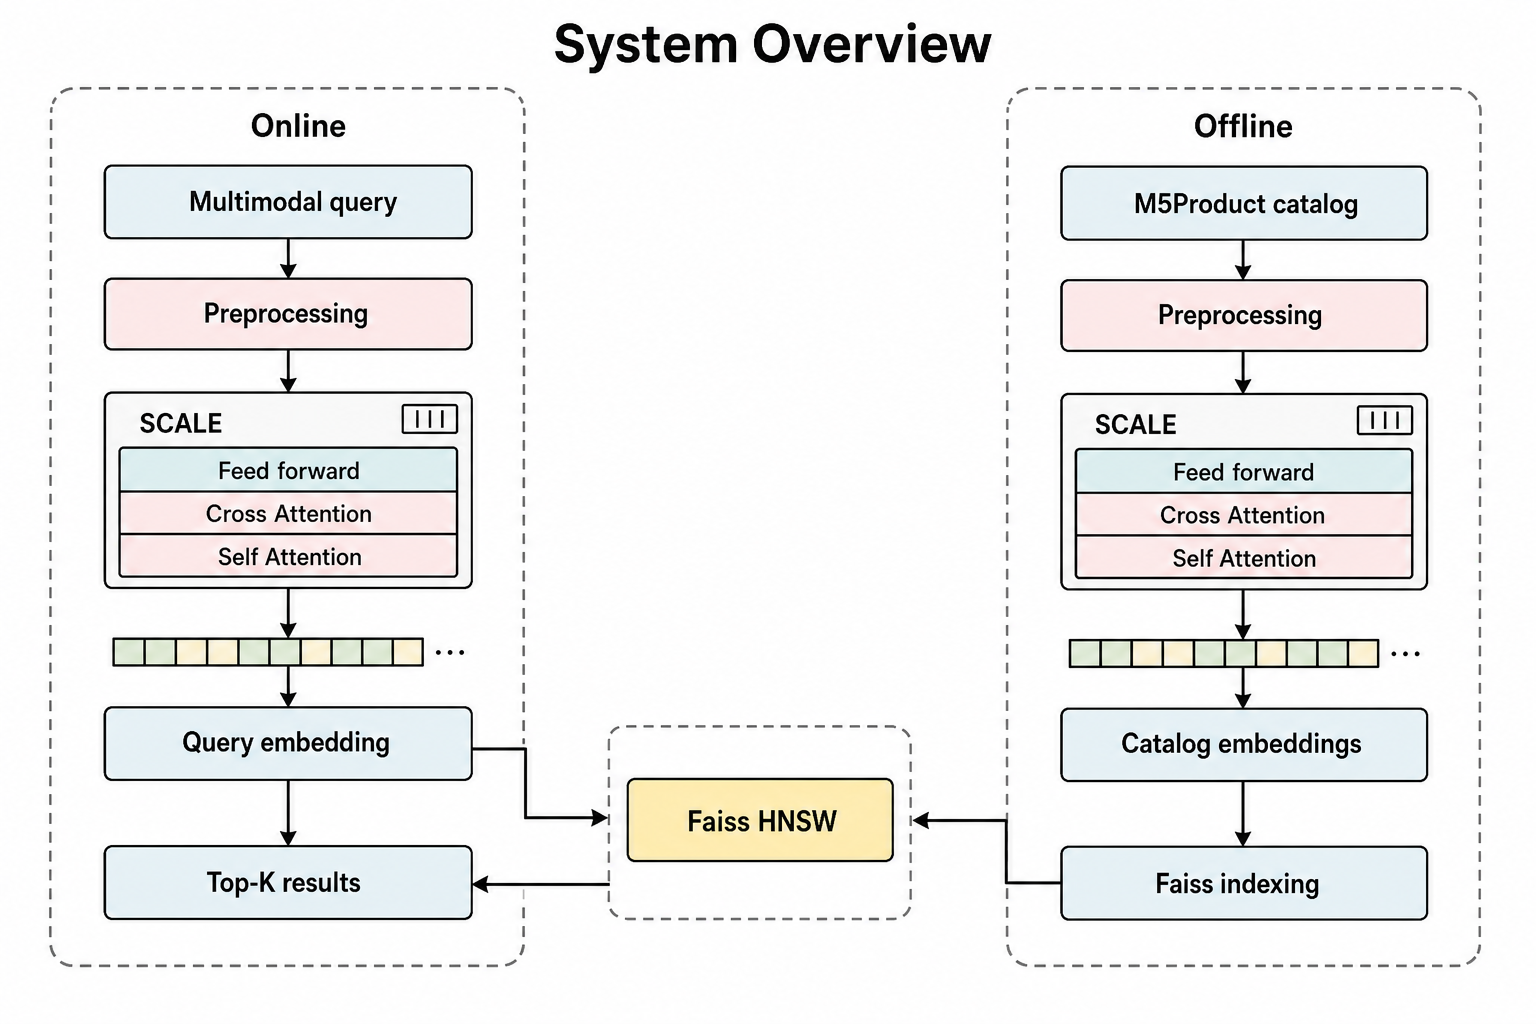
\includegraphics[width=\columnwidth]{figure/scale-faiss-pipeline.png}
\caption{Pipeline SCALE + Faiss HNSW. Offline, catalog được mã hóa và lập chỉ mục; online, query được mã hóa, truy hồi $N$ ứng viên và tái xếp hạng trước khi trả về Top-$K$.}
\label{fig:scale-faiss-pipeline}
\end{figure}

Pipeline gồm hai lớp chính: SCALE tạo unified embedding từ năm modality, còn Faiss HNSW lọc thô ứng viên và metadata reranking điều chỉnh thứ hạng cuối cùng.

\subsection{Kiến trúc SCALE}

SCALE sử dụng năm encoder cho image, text, table, video và audio. Các token được kết hợp vào Joint Co-Transformer. Kiến trúc gồm các unimodal encoder và fusion encoder, mỗi phần sử dụng sáu transformer layers với hidden size 768~\cite{dong2022m5product}. Các đoạn sau lần lượt đối chiếu phương pháp gốc với cấu hình triển khai hiện tại của từng modality.

\begin{figure*}[t]
\centering
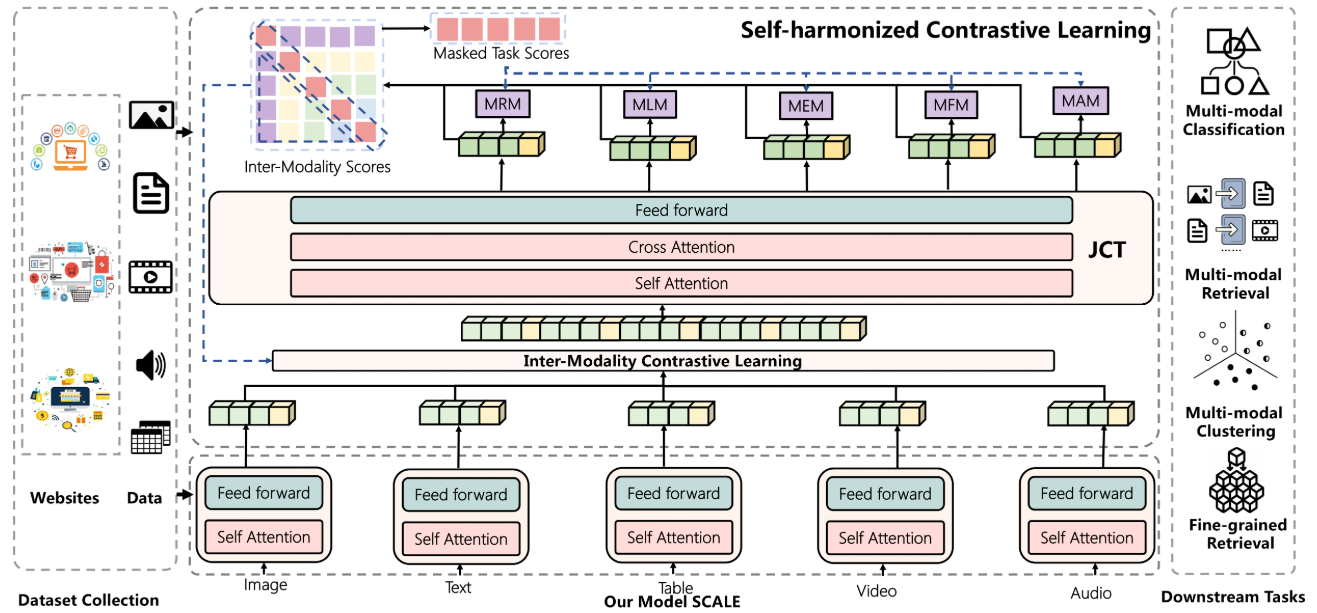
\includegraphics[width=0.85\textwidth]{figure/scale-overview.png}
\caption{Tổng quan kiến trúc SCALE: các encoder đơn phương thức được kết hợp bằng JCT, các masked tasks và SIMCL để hỗ trợ các tác vụ downstream.}
\label{fig:scale-overview}
\end{figure*}

\subsubsection{Image: region features từ Faster R-CNN}

Theo M5Product-SCALE, nhánh ảnh không đưa toàn bộ ảnh vào JCT như một tensor pixel duy nhất mà dùng region feature của Faster R-CNN ResNet-101 pretrained trên Visual Genome~\cite{ren2017faster,krishna2017visualgenome}. Từ các proposal có xác suất phát hiện lớp cao, mô hình chọn 10--36 bounding box cho mỗi ảnh. Số lượng biến thiên là cần thiết: ảnh đơn giản có thể chỉ cần vài vùng có ý nghĩa, trong khi ảnh sản phẩm chứa nhiều chi tiết cần nhiều proposal hơn. Mỗi region đi kèm tọa độ hộp và đặc trưng thị giác, nhờ đó JCT có thể tập trung vào logo, vật liệu hoặc bộ phận sản phẩm thay vì background.

Trong pipeline của đề tài, extractor dùng Detectron2 với Faster R-CNN ResNet-101 C4 và trọng số Visual Genome. Đầu ra được chuẩn hóa thành đúng 36 slot: nếu detector trả về $r<36$ vùng thì các vị trí còn lại được zero-pad và attention mask phân biệt padding với vùng thật; nếu nhiều hơn thì chỉ giữ 36 vùng điểm cao nhất. Đây là lựa chọn triển khai để tensor có kích thước cố định, không phải thay đổi phương pháp của paper.

\subsubsection{Text: BERT cho tiêu đề và caption}

Paper dùng BERT để khởi tạo text transformer, còn các transformer của modality khác được khởi tạo ngẫu nhiên. Caption được cắt ở 36 token, bao gồm token biên, để giữ chi phí self-attention thấp nhưng vẫn đủ cho title/caption ngắn của listing. BERT được chọn thay vì sentence encoder, CLIP text encoder hoặc LLM vì SCALE cần token-level representation cho MLM, attention xuyên modality trong JCT và hidden size 768 tương thích trực tiếp với backbone. Thay encoder mà không pretrain/fine-tune lại sẽ làm lệch không gian embedding và các masked task.

Source của đề tài dùng \texttt{bert-base-chinese}, một lựa chọn phù hợp với checkpoint và dữ liệu thương mại điện tử tiếng Trung của M5Product. Vì vậy, cấu hình này không nên được diễn giải là lựa chọn tối ưu cho truy vấn tiếng Việt; triển khai tiếng Việt cần dùng BERT đa ngôn ngữ hoặc mô hình tiếng Việt tương thích, sau đó huấn luyện lại các nhánh liên quan.

\subsubsection{Table: thuộc tính có cấu trúc}

Paper dùng một transformer riêng để mã hóa table, tách biệt với text transformer, và đặt chiều dài tối đa là 64 token. Table biểu diễn các cặp thuộc tính--giá trị như brand, material, color hoặc size. Trong bước chuẩn bị của đề tài, mỗi cặp được tuần tự hóa theo khuôn dạng entity--value để mô hình phân biệt rõ tên thuộc tính với giá trị. Cách biểu diễn này giữ được thông tin fine-grained mà caption thường bỏ sót; Masked Entity Modeling che cả một entity hoặc value để JCT suy luận lại từ phần table còn lại và các modality khác. Vì vậy, table đặc biệt hữu ích để phân biệt các SKU nhìn gần giống nhưng khác model, thông số hoặc thương hiệu.

\subsubsection{Video: chuỗi khung hình ngắn}

Theo paper, video gốc có tốc độ 24 FPS và chỉ lấy một frame mỗi giây để giảm thông tin dư thừa giữa các frame liền kề. Các ordinal frame này được đưa vào video encoder, sau đó tham gia JCT cùng các modality khác. Lấy mẫu theo thời gian thay vì chỉ lấy frame đầu giúp biểu diễn được nhiều góc nhìn, thao tác sử dụng hoặc trạng thái sản phẩm trong video dài.

Source hiện tại khác cấu hình paper: bộ trích xuất dùng tối đa 12 frame đầu theo thứ tự giải mã, thu nhỏ cạnh dài tối đa 480 pixel, đưa từng frame qua ResNet-50 và chuẩn hóa đầu ra về 1024 chiều; frame thiếu được zero-pad. Đây là cấu hình gọn nhẹ để tạo sidecar video trên Windows, nhưng 12 frame đầu có thể chưa bao quát toàn bộ video. Lấy mẫu đều 1 FPS và dùng video encoder như paper là hướng cải thiện cần thiết.

\subsubsection{Audio: mel-spectrogram từ 12 giây đầu}

Theo paper, audio được trích xuất từ các frame video đã chọn rồi chuyển thành đặc trưng MFCC, với frame size 1024 và hop size 256. MFCC nén phổ âm thanh theo thang Mel và phù hợp cho audio encoder cùng Masked Audio Modeling; nhánh này có thể mang thông tin từ lời thuyết minh, nhạc nền hoặc âm thanh thao tác sản phẩm. Với listing không có audio, zero imputation và attention mask giúp mô hình không diễn giải phần đệm là tín hiệu thực.

Source hiện tại dùng một biến thể gần với tiền xử lý phổ âm thanh: audio mono 16 kHz được cắt hoặc zero-pad thành 12 giây, sau đó tạo log mel-spectrogram 80 mel bins với FFT 1024, hop length 256 và chuẩn hóa theo từng mel bin, cho tensor $80\times751$. Đây là khác biệt triển khai cần được báo cáo tách biệt với MFCC của paper khi so sánh kết quả.

\begin{table}[t]
\centering
\caption{Đối chiếu tiền xử lý modality: M5Product-SCALE và source hiện tại}
\label{tab:paper-source-comparison}
\scriptsize
\renewcommand{\arraystretch}{1.12}
\begin{tabular}{L{1.0cm}L{2.75cm}L{2.85cm}}
\toprule
\textbf{Modality} & \textbf{M5Product-SCALE} & \textbf{Source hiện tại}\\
\midrule
Image & Faster R-CNN ResNet-101 trên Visual Genome; 10--36 region & Detectron2 Faster R-CNN R101 C4; chuẩn hóa 36 slot\\
Text & BERT; caption tối đa 36 token & \texttt{bert-base-chinese}; tối đa 36 token\\
Table & Transformer riêng; tối đa 64 token & Entity--value; tối đa 64 token\\
Video & Video 24 FPS, lấy 1 frame/giây & Tối đa 12 frame đầu; ResNet-50, 1024 chiều\\
Audio & MFCC; frame/hop 1024/256 & Log mel 16 kHz, 80$\times$751; FFT/hop 1024/256\\
\bottomrule
\end{tabular}
\end{table}

Bảng~\ref{tab:paper-source-comparison} cho thấy text và table giữ đúng giới hạn chuỗi của paper, trong khi image, video và audio có khác biệt ở bước trích xuất đặc trưng. Vì vậy, chỉ kết quả chạy với pipeline khớp cấu hình cột giữa mới nên được so sánh trực tiếp với các chỉ số công bố của SCALE. Các thay đổi tiền xử lý này có thể ảnh hưởng đến kết quả truy hồi cuối cùng; ảnh hưởng cụ thể được trình bày trong phần kết quả và đánh giá thực nghiệm.

\subsection{Joint Co-Transformer}

JCT là tầng hợp nhất thông tin trung tâm của SCALE. Sau các encoder riêng, mỗi modality cho một dãy token ở cùng không gian ẩn 768 chiều: $T_I$ (region ảnh), $T_T$ (caption), $T_{Tab}$ (entity--value), $T_V$ (frame video) và $T_A$ (đặc trưng audio). Với một listing thiếu modality, dãy token tương ứng được zero-impute và những vị trí đệm được đánh dấu bởi attention mask. Theo thiết kế SCALE, các dãy này không bị gộp trung bình ngay từ đầu mà được giữ ở mức token để mô hình còn có thể liên kết chi tiết giữa các modality~\cite{dong2022m5product}.

\subsubsection{Bước 1: tự chú ý trong từng modality}

Trước khi fusion, encoder riêng của mỗi modality thực hiện multi-head self-attention trên chính dãy token của modality đó. Với $X_m$ là embedding của modality $m$, mỗi head tạo query, key và value rồi tính:
\begin{equation}
\begin{aligned}
A^{\mathrm{self}}_m &=
\mathrm{softmax}\left(
\frac{(X_mW^Q_m)(X_mW^K_m)^\top}{\sqrt{d_h}}+M_m
\right),\\
Z_m &= A^{\mathrm{self}}_m(X_mW^V_m).
\end{aligned}
\end{equation}

$M_m$ che token padding hoặc modality không có dữ liệu. Bước này giúp region ảnh chọn các region ảnh liên quan khác, caption liên hệ giữa các từ, còn table/video/audio học cấu trúc nội bộ trước khi nhận tín hiệu từ nguồn khác. Mỗi khối attention được theo sau bởi residual connection, layer normalization và feed-forward network (FFN), nhờ đó đặc trưng vừa được trộn ngữ cảnh vừa giữ thông tin ban đầu.

\subsubsection{Bước 2: nối token và chú ý chéo giữa modality}

Các dãy đã mã hóa được nối thành một chuỗi chung
\begin{equation}
X=[Z_T;Z_{Tab};Z_I;Z_V;Z_A],\qquad
H=\mathrm{JCT}(X,M),
\end{equation}
trong đó $M$ là mask ghép từ năm modality. Trong JCT, self-attention được áp dụng trên toàn bộ $X$. Vì vậy, ma trận attention có các block đường chéo $A_{m,m}$ biểu diễn self-attention nội bộ và các block ngoài đường chéo $A_{m,n}$, $m\ne n$, biểu diễn cross-attention giữa hai modality:
\begin{equation}
\begin{aligned}
A_{m,n} &=
\mathrm{softmax}\left(
\frac{(Z_mW^Q)(Z_nW^K)^\top}{\sqrt{d_h}}+M_{m,n}
\right),\\
C_m &= \sum_n A_{m,n}(Z_nW^V).
\end{aligned}
\end{equation}

Nói cách khác, query của một token ảnh có thể lấy value từ token caption hoặc table; ngược lại, token text có thể tập trung vào region ảnh, frame video hay audio phù hợp. Ví dụ, token ``leather'' có thể tăng attention lên region thể hiện chất liệu da, còn token màu sắc trong table có thể điều chỉnh cách mô hình đọc ảnh sản phẩm. FFN sau attention biến đổi từng token độc lập; residual connection giữ đường truyền ổn định qua các lớp. Sau lớp JCT cuối, các dãy được tách trở lại theo ranh giới modality, pool từ token đầu mỗi dãy và kết hợp thành biểu diễn listing phục vụ masked tasks, SIMCL và retrieval.

\subsection{Học đa phương thức với cơ chế Mask (Masked Multimodal Learning)}

Masked Multimodal Learning là nhóm pretext task tự giám sát được áp dụng sau JCT. Mục tiêu không phải là dự đoán nhãn danh mục, mà buộc biểu diễn fusion phải khôi phục phần thông tin bị che từ ngữ cảnh còn lại. Với mỗi modality, SCALE che ngẫu nhiên 15\% đầu vào; phần không bị che trong cùng modality và các modality khác của \emph{cùng listing} là nguồn ngữ cảnh để tái tạo~\cite{dong2022m5product}. Hàm mất mát của modality $i$ được viết:
\begin{equation}
L_{M_i}(\theta)
=
-\mathbb{E}
\log P_\theta
(t_{\mathrm{mask}}
\mid
t_{\neg\mathrm{mask}},M_{\neg i}).
\end{equation}
Trong đó, $t_{\mathrm{mask}}$ là token hoặc feature bị che, $t_{\neg\mathrm{mask}}$ là phần chưa che của chính modality $i$, còn $M_{\neg i}$ là các modality còn lại. Vì dự đoán diễn ra sau JCT, mô hình chỉ giảm loss tốt khi đồng thời học được cấu trúc nội bộ và quan hệ liên modality, thay vì chỉ sao chép tín hiệu cục bộ.

\subsubsection{Phần bị che không phải là modality bị thiếu}

Masking là nhiễu nhân tạo, được tạo mới cho từng mẫu trong lúc pretraining; phần dữ liệu gốc \emph{không bị xóa khỏi dataset} mà được lưu riêng làm target để tính loss. Vị trí bị che vẫn giữ nguyên vị trí trong dãy token và vẫn có attention mask bằng 1, nên JCT biết rằng đó là một vị trí hợp lệ nhưng không được quan sát nội dung gốc. Điều này khác với modality thật sự không tồn tại trong listing: khi đó input được zero-impute và attention mask bằng 0 để mô hình bỏ qua toàn bộ nhánh vắng mặt.

Ở hiện thực của đề tài, cách thay thế nội dung bị che phụ thuộc vào modality. Với text, 15\% token được chọn; trong số này 80\% đổi thành \texttt{[MASK]}, 10\% đổi thành token ngẫu nhiên và 10\% giữ nguyên token gốc nhưng vẫn phải dự đoán lại. Với image region, 15\% region được chọn, trong đó 90\% feature bị thay bằng vector 0 còn 10\% được giữ nguyên để tránh mô hình chỉ phụ thuộc vào một ký hiệu mask. Video và audio thay feature của vị trí được chọn bằng vector 0. Với table, MEM chọn ngẫu nhiên một phía của cặp property--value và thay toàn bộ token của phía đó bằng \texttt{[MASK]}; phía còn lại cùng các modality khác trở thành ngữ cảnh để khôi phục. Trong mọi trường hợp, target luôn là token hoặc feature gốc trước khi thay thế.

\subsubsection{Các masked task theo modality}

\begin{itemize}[leftmargin=*]
    \item \textbf{MLM (text):} che từng word/subword trong caption và dự đoán lại token đó. Nhiệm vụ này duy trì ngữ nghĩa câu, đồng thời cho phép từ bị che nhận tín hiệu từ ảnh hoặc table.
    \item \textbf{MRP (image):} che region feature và dự đoán feature vùng ảnh tương ứng. Nhờ đó, một region bị che có thể được suy luận từ các region còn lại và mô tả sản phẩm.
    \item \textbf{MEM (table):} che toàn bộ một entity thuộc tính, chẳng hạn brand, material hoặc color, thay vì che rời rạc từng subword. Đây là điểm quan trọng vì table chứa các cặp key--value có cấu trúc; che cả entity ép mô hình khai thác quan hệ với value và các modality khác.
    \item \textbf{MFP (video):} che feature của frame được lấy mẫu và tái tạo từ các frame lân cận cùng thông tin text/image/table.
    \item \textbf{MAM (audio):} che một phần đặc trưng audio và dự đoán lại từ ngữ cảnh audio còn lại cũng như các modality đồng thời xuất hiện.
\end{itemize}

Nhãn mục tiêu của các task trên là nội dung hoặc feature gốc của phần bị che. Cách đặt bài toán chung này giúp các modality có bản chất khác nhau cùng đóng góp vào một representation space, đồng thời phù hợp với trường hợp listing thiếu modality vì attention mask ngăn JCT coi vector đệm là tín hiệu quan sát được.

\subsection{Thuật toán SIMCL}

SIMCL (Self-harmonized Inter-Modality Contrastive Learning) là thành phần căn chỉnh ngữ nghĩa giữa các modality. Với minibatch $D\in\mathbb{R}^{B\times M\times F}$, trong đó $B$ là batch size, $M$ là số modality và $F$ là chiều embedding, SCALE xét từng cặp modality $m,n$. Hai embedding $f_b^{(m)}$ và $f_b^{(n)}$ của cùng listing $b$ tạo thành một positive pair; embedding của listing khác trong batch tạo thành negative pairs. Với mỗi positive pair, có $2(B-1)$ negative pairs khi xét theo hai chiều modality.

Đặt $s_{b,r}^{m,u}=\exp(\mathrm{sim}(f_b^{(m)},f_r^{(u)})/\tau)$. Loss contrastive cho một cặp modality có dạng InfoNCE:
\begin{equation}
L_{m,n}^{CL}
=-\log
\frac{s_{b,b}^{m,n}}
{s_{b,b}^{m,n}+\displaystyle\sum_{r\ne b}\sum_{u\in\{m,n\}}s_{b,r}^{m,u}}.
\end{equation}
trong đó $\mathrm{sim}$ là cosine similarity và $\tau$ là temperature. Loss kéo các modality của cùng sản phẩm lại gần nhau, đồng thời đẩy chúng xa biểu diễn của sản phẩm khác. Tuy nhiên, không phải cặp modality nào cũng bổ trợ như nhau: image--text thường có thể hỗ trợ mạnh, trong khi audio nhiễu hoặc modality thiếu không nên nhận cùng trọng số.

\subsubsection{Tự điều hòa bằng ma trận alignment}

Để xử lý bài toán nhiều hơn hai modality, SCALE học ma trận alignment $S\in\mathbb{R}^{M\times M}$ cho từng sample. $S$ được khởi tạo từ ma trận 0 và tối ưu cùng mô hình; softmax biến các giá trị tự do thành trọng số tương đối, sau đó paper dùng phép tự điều hòa:
\begin{equation}
\widehat S=S\odot\mathrm{softmax}(S).
\end{equation}

Các phần tử tam giác trên $\widehat S^\triangle_{m,n}$ cân trọng số loss contrastive liên modality; phần tử đường chéo $\widehat S^{\mathrm{diag}}_m$ cân loss masked của từng modality. Tổng loss là:
\begin{equation}
L_{\mathrm{total}}
=
\sum_{m<n}\widehat S^\triangle_{m,n}L^{CL}_{m,n}
+
\sum_m \widehat S^{\mathrm{diag}}_m L_{M_m}.
\end{equation}

Cơ chế này khiến masked learning và contrastive learning không cạnh tranh theo trọng số cố định: mô hình tự tăng đóng góp của cặp modality có tính bổ trợ cao, đồng thời giảm ảnh hưởng của cặp ít thông tin hoặc nhiễu. Hình~\ref{fig:simcl} minh họa quá trình tạo positive/negative pairs và dùng inter-modality scores để điều hòa từng loss.

\begin{figure}[t]
\centering
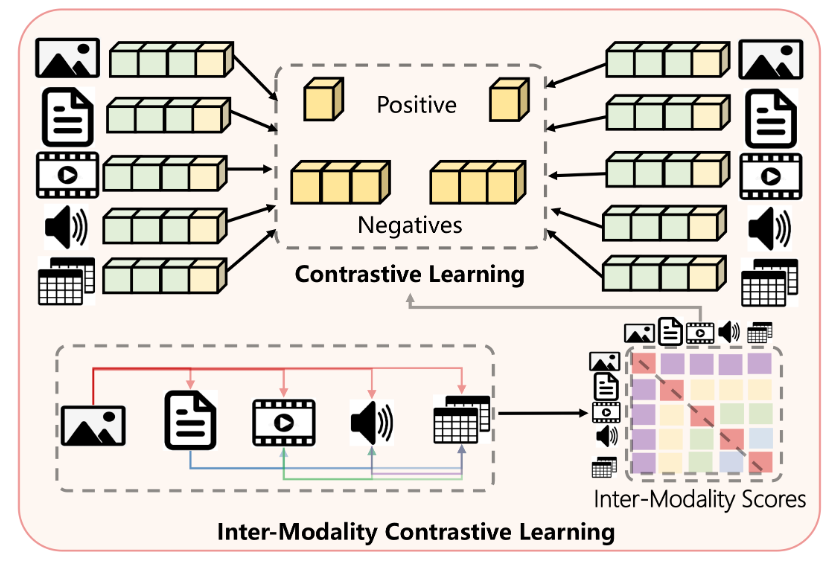
\includegraphics[width=\columnwidth]{figure/simcl.png}
\caption{Minh họa SIMCL: các cặp cùng product tạo positive pairs, các product khác tạo negatives; ma trận inter-modality scores điều chỉnh mức đóng góp của từng cặp modality.}
\label{fig:simcl}
\end{figure}

\subsection{Xử lý thiếu Modality (Missing Modality)}

Nếu một listing thiếu modality, SCALE không loại bỏ sample mà sử dụng zero imputation và attention mask. Điều này giúp mô hình vẫn học từ các listing không hoàn chỉnh và giảm ảnh hưởng của nhánh zero khi tạo embedding.

Embedding cuối cùng trong triển khai được tạo từ các pooled representation khả dụng:
\begin{equation}
e=t+p+i+v+a,
\end{equation}
sau đó được L2-normalize trước retrieval.

\subsection{Cách SCALE giải quyết hai thách thức trung tâm}

\begin{enumerate}[leftmargin=*]
    \item \textbf{Giải quyết Thách thức Modality Interaction:}
    \begin{itemize}
        \item \textbf{Kiến trúc JCT một luồng:} Nối chuỗi (concatenate) toàn bộ các token đến từ cả 5 nhánh (Image, Text, Table, Video, Audio) vào chung một khối Transformer 6 lớp. Cấu trúc này cho phép cơ chế Self-Attention hoạt động tự do trong nội bộ từng nhánh (intra-modality) lẫn xuyên suốt giữa các nhánh với nhau (cross-modality).
        \item \textbf{Ma trận căn chỉnh linh hoạt (SIMCL Alignment Matrix $S$):} Thay vì gán trọng số cố định cho mọi cặp loss liên-modality, cơ chế SIMCL khởi tạo và học một ma trận trọng số $S \in \mathbb{R}^{5 \times 5}$. Thông qua hàm Softmax, ma trận này tự động gán trọng số cao hơn cho các cặp modality bổ trợ mạnh cho nhau, đồng thời hạ thấp tầm ảnh hưởng của các cặp chứa ít thông tin hoặc chứa nhiễu.
    \end{itemize}

    \item \textbf{Giải quyết Thách thức Modality Noise (Dữ liệu không toàn vẹn):}
    \begin{itemize}
        \item \textbf{Zero Imputation:} Đối với các nhánh bị khuyết thiếu trên listing, hệ thống tự động lấp đầy (fill) các vector đầu vào bằng vector 0 (zero vector), đồng thời thiết lập các vị trí Attention Mask tương ứng bằng 0.
        \item \textbf{Học thông qua Masked Multi-modal Pretext Tasks:} Việc duy trì các mẫu thiếu trong batch huấn luyện kết hợp với các nhiệm vụ học tự giám sát (MLM, MRP, MEM, MFP, MAM) ép mô hình phải khai thác thông tin từ các modality khả dụng còn lại để khôi phục đặc trưng bị khuyết. Đồng thời, ma trận $S$ trong SIMCL cũng tự động suy giảm trọng số đối với các nhánh bị zero-impute, tránh làm lệch giá trị của hàm mất mát tổng thể.
    \end{itemize}
\end{enumerate}

% ============================================================
\section{Truy hồi với Faiss HNSW}
% ============================================================

Faiss được lựa chọn làm tầng truy hồi nhằm giải quyết trực tiếp nút thắt về chi phí tính toán trong bài toán tìm kiếm trực tuyến~\cite{johnson2019faiss}. Sau khi mô hình mã hóa chuyển đổi dữ liệu thành các vector dense đã L2-normalize, việc so sánh trực tiếp với toàn bộ catalog sẽ tốn chi phí tuyến tính $\mathcal{O}(N)$ và gây độ trễ lớn khi quy mô dữ liệu tăng cao. Faiss khắc phục vấn đề này nhờ cung cấp các cấu trúc chỉ mục tối ưu, hỗ trợ song song cả truy vấn chính xác (\textit{exact search}) để đánh giá chất lượng biểu diễn và truy vấn xấp xỉ (\textit{ANN search}). Bên cạnh đó, việc tách biệt tầng Faiss khỏi backbone còn giúp hệ thống cập nhật index linh hoạt mà không tốn chi phí huấn luyện lại mô hình gốc.

Để phục vụ catalog lớn cập nhật liên tục, đề tài tích hợp thuật toán Faiss HNSW xây dựng đồ thị tìm kiếm láng giềng xấp xỉ đa tầng, cho phép thêm sản phẩm mới trực tiếp vào chỉ mục mà không cần huấn luyện lại.

SCALE trong bài báo gốc sử dụng exact inner-product retrieval. Tuy nhiên, exact search có chi phí tăng tuyến tính theo số lượng listing. Đối với catalog lớn và cập nhật thường xuyên, đề tài bổ sung Faiss HNSW~\cite{malkov2020hnsw,johnson2019faiss}.

HNSW xây dựng đồ thị nhiều tầng cho Approximate Nearest-neighbor Search. Các tham số chính gồm $M$, $efConstruction$ và $efSearch$. Listing mới có thể được thêm vào index mà không cần huấn luyện một IVF index mới.

Quy trình online là:
\begin{enumerate}[leftmargin=*]
    \item Nhận multimodal query.
    \item Preprocess và encode bằng SCALE.
    \item L2-normalize query embedding.
    \item Tìm $N$ ứng viên bằng HNSW, với $N>K$.
    \item Tính điểm reranking trên metadata.
    \item Sắp xếp lại và trả về $K$ listing.
\end{enumerate}

HNSW chỉ là lớp serving của đề tài; các số liệu dùng để so sánh trực tiếp với paper SCALE vẫn giữ exact-retrieval protocol. Trong bản triển khai serving hiện tại, cả truy vấn Catalog ID và raw I/T/Tab đều đi qua cùng một đường: SCALE tạo query embedding, HNSW lấy $N=100$ ứng viên, sau đó một reranker dùng chung mới cắt Top-$K$. Catalog ID được tái tạo thành query I/T/Tab từ metadata và ảnh catalog, thay vì dùng một thuật toán xếp hạng riêng.


% ============================================================
\section{Tái xếp hạng dựa trên thuộc tính (Attribute-aware Reranking)}
% ============================================================

\subsection{Động lực và Hạn chế của Retrieval Thuần Embedding}

Embedding similarity ($S_{\mathrm{emb}}$) thu được từ không gian ẩn của SCALE đóng vai trò rất tốt trong việc bắt các đặc trưng tổng thể. Tuy nhiên, phương pháp retrieval thuần embedding gặp phải ba hạn chế cốt lõi trong thực tế thương mại điện tử:
\begin{enumerate}[leftmargin=*]
    \item \textbf{Hiện tượng trùng lặp đặc trưng thị giác khác ngành:} Các sản phẩm thuộc các danh mục hoàn toàn khác nhau có thể sở hữu vẻ ngoài tương đồng (ví dụ: một chiếc ốp điện thoại hình bao da có hoa văn chất liệu da rất dễ có vector embedding gần với một chiếc ví cầm tay da).
    \item \textbf{Nhiễu nền và thành phần phụ:} Ảnh sản phẩm e-commerce thường chứa chữ quảng cáo, logo thương hiệu, watermark hoặc mẫu nhân vật (model). Điều này khiến vector embedding bị lệch khỏi đối tượng chính.
    \item \textbf{Bỏ sót thuộc tính quyết định:} Độ tương đồng vector chỉ phản ánh sự gần giống, nhưng giao dịch e-commerce yêu cầu sự chính xác tuyệt đối về các thuộc tính cứng như thương hiệu (Brand), siêu danh mục (Super-category) hoặc danh mục chi tiết (Category).
\end{enumerate}

Để giảm các lỗi này, tầng tái xếp hạng metadata được tích hợp ngay sau bước lọc thô của Faiss HNSW. Bản serving hiện tại dùng title và PV attributes làm metadata quan sát được; không dùng siêu danh mục, category hay product label vì các trường đó không có ở raw query và không được phép rò rỉ vào đánh giá.

\subsection{Reranking dùng chung cho Catalog ID và Raw Query}

Sau khi HNSW trả về cùng tập $N$ ứng viên, hệ thống tạo văn bản metadata bằng phép nối title và PV attributes. $S_{\mathrm{attr}}(q,p_i)$ là cosine similarity giữa các vector TF--IDF character $2$--$3$ gram của văn bản query và ứng viên. Cách này dùng được cho cả Catalog ID (metadata của listing) lẫn raw query (text/table người dùng nhập), không cần suy luận nhãn, super-category hay category từ gallery.

Với truy vấn image-only không có text/table, $S_{\mathrm{attr}}=0$; thứ hạng chỉ dựa trên $S_{\mathrm{emb}}$. Do đó hệ thống không dùng majority voting hoặc bất kỳ product label nào trong serving. Đây là giới hạn có chủ đích để không làm rò rỉ nhãn đánh giá vào kết quả truy hồi.

\subsection{Hàm Điểm Tổng hợp và Điều chỉnh Miền}

Điểm số cuối cùng dùng để sắp xếp lại danh sách kết quả trước khi cắt lấy Top-$K$ được tính theo công thức kết hợp tuyến tính:

\begin{equation}
S_{\mathrm{total}}(q, p_i) = \lambda \cdot S_{\mathrm{emb}}(q, p_i) + (1 - \lambda) \cdot S_{\mathrm{attr}}(q, p_i),
\end{equation}
với $\lambda=0.7$ trong cấu hình serving hiện tại. Cùng một giá trị và cùng công thức được áp dụng cho mọi ngành hàng, cho Catalog ID và raw query. Các trọng số theo miền sản phẩm là hướng thử nghiệm trong tương lai, không phải kết quả đã triển khai hay đã đánh giá.

\subsection{So sánh với reranking Catalog ID trước đây}

Phiên bản serving trước đây chỉ áp dụng reranking cho Catalog ID. Nó so sánh trực tiếp embedding đã lưu với \emph{toàn bộ} gallery để có $S_{\mathrm{exact}}$, sau đó trộn mạnh với TF--IDF title/PV:
\begin{equation}
S_{\mathrm{old}}(q,p_i)=0.25\,S_{\mathrm{exact}}(q,p_i)+0.75\,S_{\mathrm{attr}}(q,p_i).
\end{equation}
Raw query ở phiên bản đó không dùng công thức trên: nó chỉ trả kết quả FAISS theo $S_{\mathrm{emb}}$. Vì vậy, cùng một sản phẩm khi truy vấn bằng Catalog ID hoặc nhập raw I/T/Tab có thể có candidate set, trọng số và thứ hạng khác nhau.

Cấu hình hiện tại thay bằng một công thức chung sau khi HNSW trả về $N=100$ ứng viên:
\begin{equation}
\begin{aligned}
S_{\mathrm{new}}(q,p_i) &= 0.70\,S_{\mathrm{emb}}(q,p_i) \\
&\quad + 0.30\,S_{\mathrm{attr}}(q,p_i), \\
p_i &\in \operatorname{TopN}_{\mathrm{HNSW}}(q).
\end{aligned}
\end{equation}

Hướng mới được chọn vì ba lý do. Thứ nhất, Catalog ID và raw query có cùng candidate set, cùng metadata score và cùng công thức, nên hai cách kiểm thử đối chiếu được khi đầu vào I/T/Tab tương đương. Thứ hai, HNSW thực hiện bước lọc theo đúng kiến trúc serving của báo cáo, thay vì Catalog ID âm thầm thực hiện full-scan khác với raw query. Thứ ba, trọng số embedding $0.70$ giữ SCALE là tín hiệu chính; title/PV chỉ điều chỉnh thứ hạng trong tập ứng viên gần, giảm rủi ro lexical overlap lấn át representation đa phương thức. Đây là quyết định thiết kế để đảm bảo nhất quán, không phải tuyên bố rằng $0.70/0.30$ đã tối ưu; benchmark tái lập mới là điều kiện để chọn trọng số cuối cùng.



% ============================================================
\section{Thiết lập thực nghiệm}
% ============================================================

\subsection{Cấu hình huấn luyện}

\begin{table}[t]
\centering
\caption{Cấu hình chính}
\label{tab:config}
\small
\begin{tabular}{L{2.25cm}L{4.45cm}}
\toprule
\textbf{Thành phần} & \textbf{Thiết lập}\\
\midrule
Tập dữ liệu & M5Product subset\\
Số lượng mẫu & 10,000\\
Phân bố & 70/20/10\\
Kiến trúc & SCALE\\
Hidden size & 768\\
Độ dài Văn bản & 36\\
Độ dài Bảng & 64\\
Vùng ảnh (Paper / source) & 10--36 region / 36 slot cố định\\
Video (Paper / source) & 1 frame/giây từ 24 FPS / 12 frame đầu, ResNet-50\\
Audio (Paper / source) & MFCC / log mel-spectrogram ($80\times751$)\\
Tỷ lệ Masking & 15\%\\
Số epoch (bài báo gốc) & 5 epochs\\
Số epoch (pipeline dự kiến) & 10 epochs\\
Bộ tối ưu & Adam\\
Learning rate (Gốc) & $10^{-4}$\\
Phần cứng (Gốc) & 4 GPUs\\
\bottomrule
\end{tabular}
\end{table}

Các cấu hình trong Bảng~\ref{tab:config} mô tả pipeline thiết kế. Kết quả thực nghiệm hiện có chỉ lưu các metric của đặc trưng năm modality; vì vậy chúng không đủ để khẳng định checkpoint, seed, số mẫu thực tế hay tham số HNSW. Các thông tin này cần được lưu kèm mỗi lần chạy để bảo đảm tái lập.

\subsection{Đánh giá truy hồi (Retrieval Evaluation)}

Để so sánh trực tiếp với kết quả SCALE, cần giữ nguyên pipeline gốc:
\begin{enumerate}[leftmargin=*]
    \item Trích xuất pooled embeddings;
    \item Tính exact score $q^\top G$;
    \item Loại query khỏi ranking;
    \item Lấy tối đa 10 kết quả;
    \item Đánh giá với ground truth category.
\end{enumerate}

Các metric chính là mAP@1, mAP@5, mAP@10 và Precision@1, Precision@5, Precision@10. Mỗi lần chạy phải lưu cách xác định positive set và công thức AP. Với tập con tự tạo, positive set theo nhãn nội bộ không phải ground truth chính thức của M5Product; do đó không được đặt hai loại kết quả trên cùng một thang so sánh.

HNSW, latency, QPS, recall so với FlatIP và thời gian thêm listing cần được đánh giá riêng như system-level metrics, không trộn với bảng representation của SCALE.

% ============================================================
\section{Kết quả và Đánh giá thực nghiệm}
% ============================================================

\subsection{Kết quả tham chiếu từ SCALE}

Bảng~\ref{tab:scale-results} trình bày các số liệu tham chiếu được báo cáo trong tài liệu SCALE trên subset của M5Product. Mỗi cặp là pretrain/finetune.

\begin{table*}[t]
\centering
\caption{Kết quả tham chiếu SCALE khi tăng số modality}
\label{tab:scale-results}
\small
\begin{tabular}{lrrrrrrr}
\toprule
\textbf{Modality} & \textbf{Acc.} & \textbf{mAP@1} & \textbf{mAP@5} &
\textbf{mAP@10} & \textbf{Prec@1} & \textbf{Prec@5} & \textbf{Prec@10}\\
\midrule
Text & 77.42 & 47.70/65.10 & 53.63/68.39 & 51.59/66.99 & 47.70/65.10 & 30.96/44.89 & 24.15/33.44\\
+Image & 79.58 & 51.47/67.02 & 56.16/69.85 & 54.41/68.43 & 51.47/67.02 & 33.41/46.29 & 25.55/34.29\\
+Table & 82.83 & 57.14/67.97 & 61.71/70.34 & 59.64/69.38 & 57.14/67.97 & 38.02/46.85 & 28.99/34.36\\
+Video & 84.31 & 58.57/69.79 & 63.15/72.30 & 61.02/70.67 & 58.57/69.79 & 39.26/47.44 & 29.56/34.78\\
+Audio & 85.50 & 58.72/70.62 & 63.17/73.02 & 61.05/71.50 & 58.72/70.62 & 39.66/48.20 & 30.32/35.35\\
\bottomrule
\end{tabular}
\end{table*}

Trên subset được báo cáo trong tài liệu gốc, việc bổ sung modality nhìn chung cải thiện Accuracy và retrieval metrics. Năm modality đạt Accuracy 85.50 và mAP@1 58.72/70.62.

\subsection{Metric representation theo bài toán gốc}

Hai bảng sau cùng thuộc bài toán representation retrieval: query TPIVA được so với gallery TPIVA, không dùng title/PV reranking. Bảng~\ref{tab:scale-results} là kết quả do SCALE công bố theo M5Product protocol. Bảng~\ref{tab:local-results} là kết quả tái lập nội bộ bằng script retrieval gốc: dot product trực tiếp trên TPIVA test và gallery, sau đó chấm positive cùng label trong subset. Hai bảng phải được đặt cạnh nhau để tham chiếu, nhưng không được so sánh như hai benchmark đồng nhất vì khác checkpoint, quy mô dữ liệu, positive definition và protocol ground truth.

\begin{table}[t]
\centering
\caption{Tái lập nội bộ metric representation gốc (\%)}
\label{tab:local-results}
\small
\begin{tabular}{crrr}
\toprule
$K$ & mAP & Precision & HitRate\\
\midrule
1  & 0.19 & 0.19 & 0.19\\
5  & 0.39 & 0.28 & 1.42\\
10 & 0.45 & 0.25 & 2.47\\
\midrule
Trung bình @1/@5/@10 & 0.34 & 0.24 & --\\
\bottomrule
\end{tabular}
\end{table}

Ở $K=10$, tái lập nội bộ đạt mAP 0.45\% và Precision 0.25\%. Đây là số liệu của representation-only protocol hiện có, không phải kết quả của pipeline serving.

\subsection{Metric hệ thống cho pipeline serving}

Ngược lại, Bảng~\ref{tab:serving-results} đo bài toán hệ thống của đề tài: 1,054 TPIVA test query được L2-normalize, HNSW lấy 100 ứng viên, sau đó title/PV TF--IDF reranking với $\lambda=0.7$ mới trả Top-$K$. Label chỉ được dùng ở bước chấm điểm positive cùng label, không được đưa vào retrieval hoặc reranking. Paper SCALE không công bố metric cho pipeline HNSW + metadata này nên bảng chỉ có kết quả của hệ thống hiện tại.

\begin{table}[t]
\centering
\caption{Metric pipeline serving HNSW + reranking dùng chung (\%)}
\label{tab:serving-results}
\small
\begin{tabular}{crrr}
\toprule
$K$ & mAP & Precision & HitRate\\
\midrule
1  & 16.13 & 16.13 & 16.13\\
5  & 12.48 & 4.90 & 20.59\\
10 & 12.54 & 2.63 & 22.20\\
\midrule
Trung bình @1/@5/@10 & 13.72 & 7.88 & --\\
\bottomrule
\end{tabular}
\end{table}

\subsubsection{Vì sao hai nhóm metric chênh lệch lớn}

Chênh lệch không phải do chỉ thay cách tính metric, mà do ba thay đổi của hệ thống xếp hạng. (i) Script gốc dùng dot product không L2-normalize; norm TPIVA trong lần chạy này dao động từ 270 đến 342, nên độ lớn vector ảnh hưởng mạnh đến thứ hạng. Khi L2-normalize và chỉ dùng HNSW embedding-only, mAP@10 tăng từ 0.45\% lên 2.10\%. (ii) Serving HNSW sử dụng candidate set cố định 100 item, thay vì full-scan theo dot product cũ. (iii) Reranker dùng title/PV là tín hiệu quan sát được của query và nâng mAP@10 tiếp từ 2.10\% lên 12.54\%. Vì vậy mức tăng là thay đổi retrieval objective từ representation-only sang multimodal serving, không phải bằng chứng rằng backbone SCALE tự tăng tương ứng.

Ở Top-1, mAP tăng từ 0.19\% lên 16.13\%, xấp xỉ 85 lần; ở Top-10, tăng từ 0.45\% lên 12.54\%, xấp xỉ 28 lần. Sự tăng này hợp lý vì title/PV trong M5Product thường chứa brand, model và thuộc tính phân biệt trực tiếp; tuy nhiên nó phải được diễn giải là hiệu năng của pipeline có metadata, không được dùng để so sánh trực tiếp với metric original của SCALE.

\subsubsection{Vì sao metric nội bộ thấp hơn kết quả công bố}

Không nên so sánh trực tiếp Bảng~\ref{tab:local-results} với kết quả SCALE trong paper như hai benchmark đồng nhất. Paper huấn luyện SCALE trên M5Product quy mô lớn, sử dụng protocol, positive definition, pretraining và fine-tuning riêng~\cite{dong2022m5product}; trong khi thí nghiệm nội bộ dùng subset 10,000 mẫu được chia 70/20/10. Subset nhỏ làm giảm độ đa dạng category, số biến thể của cùng sản phẩm và số positive/negative quan sát trong huấn luyện, đồng thời làm metric nhạy hơn với từng query và seed. Phân bố sau lấy mẫu, cách tạo gallery/query và cách xác định cùng sản phẩm cũng có thể khác protocol coarse- hoặc fine-grained retrieval của paper.

\subsubsection{Ảnh hưởng của pipeline hiện thực}

Khác biệt hiện thực ảnh hưởng trực tiếp đến distribution của feature mà SCALE nhìn thấy. Ở nhánh ảnh, pipeline luôn đưa 36 region vào encoder. Cấu hình này giúp tensor có kích thước cố định và thuận lợi cho batch processing, nhưng khác với việc paper chọn linh hoạt 10--36 proposal có độ tin cậy cao. Khi ảnh chỉ có ít vùng sản phẩm có ý nghĩa, các slot còn lại là padding; ngược lại, ảnh phức tạp có thể có nhiều proposal hợp lệ nhưng chỉ 36 vùng điểm cao nhất được giữ lại. Vì vậy, chất lượng region feature và attention mask trở nên rất nhạy với detector cũng như đặc điểm ảnh thương mại điện tử có chữ quảng cáo, logo hoặc nhiều sản phẩm trong cùng khung hình.

Khác biệt rõ hơn nằm ở tín hiệu thời gian. Paper lấy mẫu đều một frame mỗi giây từ video 24 FPS để bao phủ toàn bộ diễn tiến, còn pipeline hiện tại dùng tối đa 12 frame đầu theo thứ tự giải mã. Nếu phần giới thiệu, thao tác sử dụng hoặc góc quay quan trọng nằm ở nửa sau video, representation video hiện tại không quan sát được tín hiệu đó. Tương tự, log mel-spectrogram giữ năng lượng theo các dải tần Mel, trong khi MFCC nén phổ theo hệ số cepstral. Hai biểu diễn có kích thước và phân bố khác nhau; do đó audio encoder hoặc masked-audio head được huấn luyện theo một cách biểu diễn không thể được xem là tương đương trực tiếp với cấu hình MFCC của paper.

\subsubsection{Giới hạn đánh giá end-to-end}

Để metric phản ánh đúng năng lực SCALE, query mới và catalog phải được mã hóa bởi cùng checkpoint, cùng tiền xử lý và cùng không gian embedding. Serving hiện tại đã mã hóa raw query trực tiếp bằng checkpoint SCALE; Catalog ID được tái tạo thành cùng query I/T/Tab và đi qua cùng HNSW cùng reranker. Tuy nhiên, cosine giữa online preprocessing và feature offline cần tiếp tục được theo dõi bằng smoke test, đồng thời cần lưu log candidate trước/sau reranking và manifest tham số để quy kết mức tăng metric.

Vì vậy, metric thấp hơn không đồng nghĩa SCALE kém hơn kết quả công bố. Chúng phản ánh tổng hợp khác biệt về quy mô dữ liệu, protocol, positive definition, pipeline tiền xử lý, checkpoint pretraining/fine-tuning và mức hoàn thiện hệ thống. Một manifest đầy đủ cho mỗi lần chạy, gồm split, seed, số query, checkpoint, tham số HNSW, trọng số reranking và latency, là điều kiện cần để xác định phần chênh lệch nào đến từ representation, phần nào đến từ serving.

\FloatBarrier

% ============================================================
\section{Thảo luận}
% ============================================================

\subsection{Tương tác giữa các Modality}

Mỗi modality mô tả một phần khác nhau của sản phẩm. Image cung cấp appearance, text cung cấp semantic intent, table chứa thông tin fine-grained, video cung cấp use case và audio bổ sung lời giới thiệu. JCT cho phép các nguồn thông tin này tương tác, trong khi SIMCL tránh việc gán trọng số đồng đều cho mọi cặp modality.

\subsection{Thiếu Modality}

Zero imputation cho phép mẫu thiếu modality vẫn được giữ trong training và catalog. Đây là yếu tố quan trọng đối với e-commerce vì listing không phải lúc nào cũng có đủ ảnh, text, table, video và audio. Tuy nhiên, nếu một query hoặc một catalog item chỉ có rất ít tín hiệu, embedding có thể kém phân biệt.

\subsection{Nhiễu thị giác (Visual Noise)}

Ảnh listing thường có chữ quảng cáo, watermark, logo shop, người, vật tặng hoặc nhiều biến thể trong cùng frame. Region feature của Faster R-CNN giảm một phần vấn đề nhưng chưa đảm bảo loại bỏ hoàn toàn background và object phụ. Metadata reranking được thiết kế để xử lý một phần lỗi fine-grained sau bước retrieval.

\subsection{Giới hạn hiện thực và khả năng suy diễn}

Phần đánh giá dùng label chỉ để chấm positive, không dùng label để xếp hạng. API hiện đã có encoder raw query và reranking end-to-end: cùng HNSW candidate set, TF--IDF title/PV và $\lambda=0.7$ cho Catalog ID lẫn raw query. Benchmark serving đã được lưu cùng tham số và split; tuy nhiên chưa có candidate logs hoặc ablation đầy đủ, nên Bảng~\ref{tab:serving-results} không được dùng để khẳng định riêng mức đóng góp của reranking.

% ============================================================
\section{Hướng phát triển tương lai}
% ============================================================

Ba hướng ưu tiên để hoàn thiện hệ thống là:
\begin{itemize}[leftmargin=*]
    \item \textbf{Ablation và tái lập có kiểm soát:} đánh giá lần lượt SCALE exact retrieval, SCALE + HNSW, và SCALE + HNSW + metadata reranking trên cùng split; sau đó tách các nhóm query image-only, image+text và có table. Ablation theo số modality, nhiều seed, cùng manifest gồm checkpoint, split, positive definition, tham số index và trọng số reranking sẽ cho biết chính xác thành phần nào tạo ra mức tăng.
    \item \textbf{Tích hợp pipeline chuẩn SCALE:} thay các bước được đơn giản hóa do giới hạn phần cứng bằng cấu hình sát paper hơn: sampling video 1 frame/giây, audio MFCC, feature extractor và checkpoint pretraining/fine-tuning tương thích. Mục tiêu là để representation của query và catalog được tạo bởi cùng pipeline SCALE, từ đó so sánh công bằng hơn với kết quả công bố.
\end{itemize}

% ============================================================
\section{Kết luận}
% ============================================================

Bài báo trình bày hệ thống multimodal retrieval cho catalog thương mại điện tử: SCALE tạo biểu diễn năm modality, Faiss HNSW sinh candidate và reranker không dùng nhãn trộn điểm embedding với title/PV metadata. Catalog ID và raw I/T/Tab dùng cùng một đường serving, nên có thể đối chiếu trực tiếp khi đầu vào tương đương.

Đóng góp chính của bản báo cáo là tách bạch ba mức bằng chứng: số liệu tham chiếu từ paper SCALE, metric representation tái lập nội bộ và metric của hệ thống end-to-end hiện tại. Bước tiếp theo là lưu candidate logs và chạy ablation exact retrieval, HNSW embedding-only và HNSW + reranking trên cùng split.


\section*{Lời cảm ơn}
Nhóm xin chân thành cảm ơn TS. Võ Hoài Việt đã truyền đạt những kiến thức chuyên môn quý báu và mang đến những bài giảng ý nghĩa. Thầy cũng là người đã nhiệt tình hướng dẫn, giải đáp các thắc mắc đồng thời đóng góp nhiều ý kiến giá trị từ hình thức trình bày đến nội dung chuyên môn sao cho hợp lý góp phần giúp nhóm hoàn thiện báo cáo này.

Mặc dù đã cố gắng hoàn thành đồ án một cách tốt nhất nhưng bài báo cáo khó có thể tránh khỏi những hạn chế thiếu sót và nhóm rất mong nhận được sự thông cảm và góp ý từ Thầy. 



% ============================================================
% REFERENCES
% ============================================================
% Cân đều hai cột ở trang tài liệu tham khảo cuối cùng.
\renewcommand{\refname}{Tài liệu tham khảo}
\balance

\begin{thebibliography}{99}

\bibitem{venkatesan2025}
N. Venkatesan, M. Suresh, V. R. Paul, D. K. Das, and P. Vijayakumar,
``The Rise of Visual Search in E-Commerce: Leveraging AI to Redefine Product Discovery,''
Journal of Marketing \& Social Research, 2025.

\bibitem{dong2022m5product}
X. Dong, X. Zhan, Y. Wu, Y. Wei, M. C. Kampffmeyer, X.-Y. Wei,
M. Lu, Y. Wang, and X. Liang,
``M5Product: Self-harmonized Contrastive Learning for E-commercial Multi-modal Pretraining,''
2022.

\bibitem{nadkarni2022shopsy}
P. Nadkarni and N. V. Dasararaju,
``Visually Similar Products Retrieval for Shopsy,''
arXiv:2210.04560, 2022.

\bibitem{liu2024miem}
C. Liu, P. Hou, A. Zeng, and H. Yu,
``Transformer-Empowered Multi-Modal Item Embedding for Enhanced Image Search in E-commerce,''
in \emph{Proc. AAAI}, 2024.

\bibitem{jiang2024mrse}
H. Jiang, H. Zhang, Q. Hou, C. Chen, W. Lin, J. Zhang, and A. Wang,
``MRSE: An Efficient Multi-modality Retrieval System for Large Scale E-commerce,''
2024.

\bibitem{yuan2026fashionmv}
P. Yuan, B. Mei, and H. Zhang,
``FashionMV: Product-Level Composed Image Retrieval with Multi-View Fashion Data,''
arXiv:2604.10297, 2026.

\bibitem{ren2017faster}
S. Ren, K. He, R. Girshick, and J. Sun,
``Faster R-CNN: Towards Real-Time Object Detection with Region Proposal Networks,''
\emph{IEEE Trans. Pattern Anal. Mach. Intell.}, 2017.

\bibitem{he2016resnet}
K. He, X. Zhang, S. Ren, and J. Sun,
``Deep Residual Learning for Image Recognition,''
in \emph{Proc. CVPR}, 2016.

\bibitem{devlin2019bert}
J. Devlin, M.-W. Chang, K. Lee, and K. Toutanova,
``BERT: Pre-training of Deep Bidirectional Transformers for Language Understanding,''
in \emph{Proc. NAACL-HLT}, 2019.

\bibitem{radford2021clip}
A. Radford et al.,
``Learning Transferable Visual Models From Natural Language Supervision,''
in \emph{Proc. ICML}, 2021.

\bibitem{malkov2020hnsw}
Y. A. Malkov and D. A. Yashunin,
``Efficient and Robust Approximate Nearest Neighbor Search Using Hierarchical Navigable Small World Graphs,''
\emph{IEEE Trans. Pattern Anal. Mach. Intell.}, 2020.

\bibitem{johnson2019faiss}
J. Johnson, M. Douze, and H. Jégou,
``Billion-scale similarity search with GPUs,''
\emph{IEEE Trans. Big Data}, 2019.

\bibitem{dosovitskiy2021vit}
A. Dosovitskiy et al.,
``An Image is Worth 16x16 Words: Transformers for Image Recognition at Scale,''
in \emph{Proc. ICLR}, 2021.

\bibitem{anderson2018bottomup}
P. Anderson et al.,
``Bottom-Up and Top-Down Attention for Image Captioning and Visual Question Answering,''
in \emph{Proc. CVPR}, 2018.

\bibitem{krishna2017visualgenome}
R. Krishna et al.,
``Visual Genome: Connecting Language and Vision Using Crowdsourced Dense Image Annotations,''
\emph{Int. J. Comput. Vis.}, 2017.

\bibitem{vaswani2017attention}
A. Vaswani et al.,
``Attention Is All You Need,''
in \emph{Advances in Neural Information Processing Systems}, 2017.

\bibitem{davis1980mfcc}
S. Davis and P. Mermelstein,
``Comparison of Parametric Representations for Monosyllabic Word Recognition in Continuously Spoken Sentences,''
\emph{IEEE Trans. Acoust., Speech, Signal Process.}, 1980.

\bibitem{faissdocs}
Meta AI,
``Faiss Documentation.''
[Online]. Available: \url{https://faiss.ai/}

\bibitem{pytorch}
PyTorch Contributors,
``PyTorch.''
[Online]. Available: \url{https://pytorch.org/}

\bibitem{transformers}
Hugging Face,
``Transformers Documentation.''
[Online]. Available: \url{https://huggingface.co/docs/transformers}

\bibitem{librosa}
Librosa Developers,
``librosa Documentation.''
[Online]. Available: \url{https://librosa.org/doc/latest/}

\bibitem{ffmpeg}
FFmpeg Developers,
``FFmpeg Documentation.''
[Online]. Available: \url{https://ffmpeg.org/documentation.html}

\end{thebibliography}

% ============================================================
% APPENDIX
% ============================================================

\clearpage
\onecolumn
\renewcommand{\appendixname}{Phụ lục}
\appendices
\section{Danh mục ký hiệu}
\label{app:notation}

\begin{table}[htbp]
\centering
\caption{Các ký hiệu sử dụng trong báo cáo}
\label{tab:notation}
\small
\renewcommand{\arraystretch}{1.16}
\setlength{\tabcolsep}{7pt}
\begin{tabular}{L{4.0cm} L{12.8cm}}
\toprule
\textbf{Ký hiệu} & \textbf{Ý nghĩa} \\
\midrule
$q = (I, T, Tab, V, A)$ & Query đa phương thức (Image, Text, Table, Video, Audio); có thể chỉ có một modality. \\
$G = \{p_1, \ldots, p_N\}$ & Kho sản phẩm. \\
$p_i$ & Một listing, cùng bộ năm modality, có thể thiếu nhánh. \\
$K$ & Số kết quả trả về. \\
$N$ & Số ứng viên lọc thô HNSW; serving hiện tại dùng $N=100$. \\
$f(\cdot)$ & SCALE encoder, unified embedding. \\
$\mathrm{sim}(\cdot) / S_{\mathrm{emb}}$ & Độ tương đồng embedding (inner product sau L2-normalize). \\
$S$ & Alignment score matrix trong SIMCL. \\
$S(u, v)$ & Mức bổ trợ semantic giữa hai modality. \\
$S_{\mathrm{attr}}$ & Cosine TF--IDF character n-gram giữa title/PV của query và candidate. \\
$S_{\mathrm{total}}$ & $\lambda S_{\mathrm{emb}} + (1-\lambda) S_{\mathrm{attr}}$, với $\lambda=0.7$. \\
$\mathrm{JCT}$ & Joint Co-Transformer. \\
$\mathrm{SIMCL}$ & Self-harmonized Inter-Modality Contrastive Learning. \\
$\mathrm{HNSW}$ & Hierarchical Navigable Small World (Faiss). \\
\bottomrule
\end{tabular}
\end{table}

\clearpage
\section{Giao diện hệ thống}
\label{app:frontend}

Phụ lục này minh họa giao diện của hệ thống retrieval trong ba trạng thái sử dụng
chính: nhập truy vấn đa phương thức, tìm kiếm theo Catalog ID và xem chi tiết sản
phẩm. Hai màn hình tìm kiếm được đặt cạnh nhau để thuận tiện đối chiếu; màn hình
chi tiết được trình bày riêng ở phía dưới.

\begin{figure}[htbp]
    \centering
    \begin{minipage}[t]{0.485\textwidth}
        \centering
        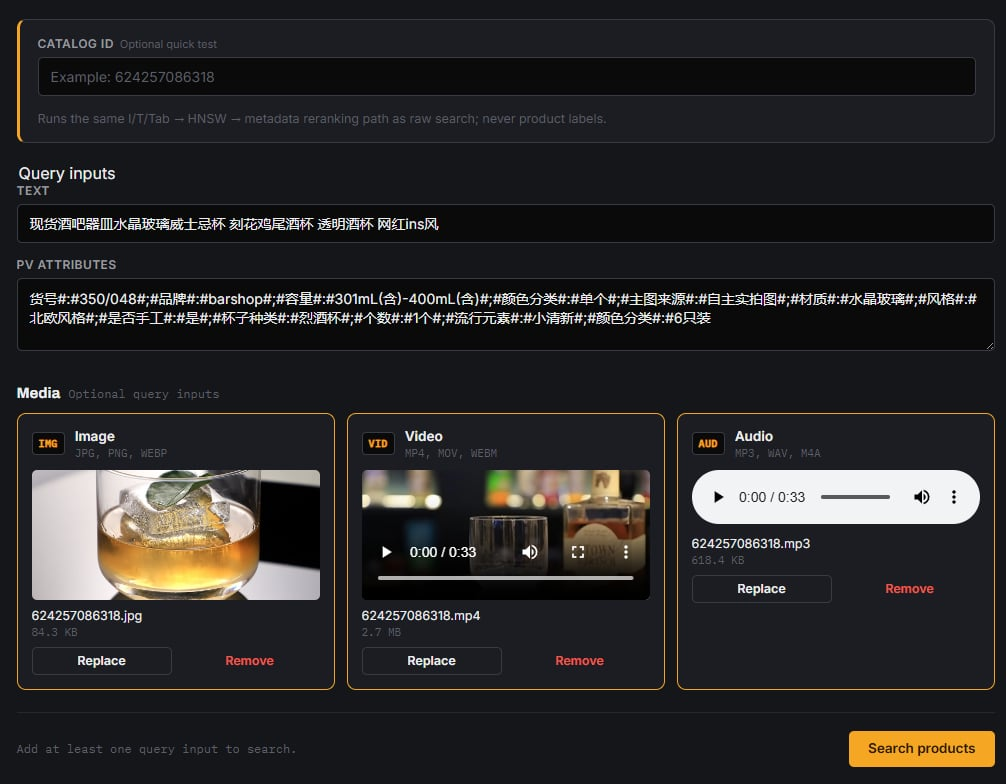
\includegraphics[width=\linewidth]{figure/fe1.jpg}
        \vspace{2pt}

        \small (a) Nhập truy vấn raw bằng text và PV attributes.
    \end{minipage}\hfill
    \begin{minipage}[t]{0.485\textwidth}
        \centering
        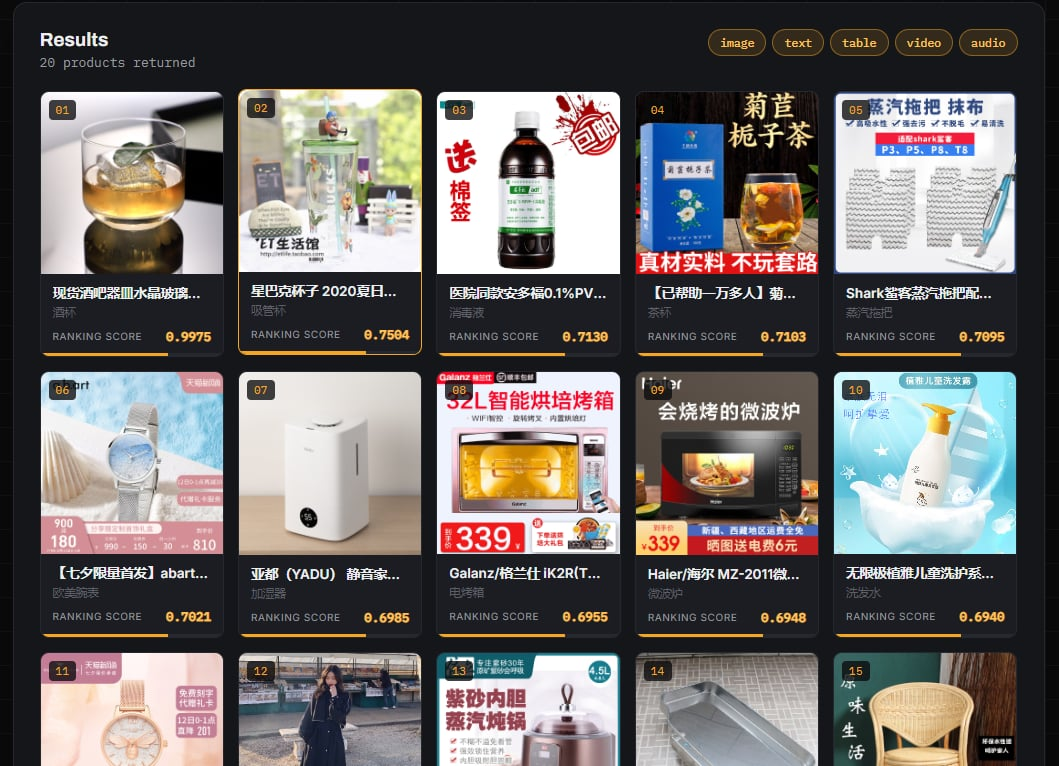
\includegraphics[width=\linewidth]{figure/fe2.jpg}
        \vspace{2pt}

        \small (b) Tìm kiếm theo Catalog ID và hiển thị kết quả Top-$K$.
    \end{minipage}

    \vspace{0.7em}

    \begin{minipage}[t]{0.68\textwidth}
        \centering
        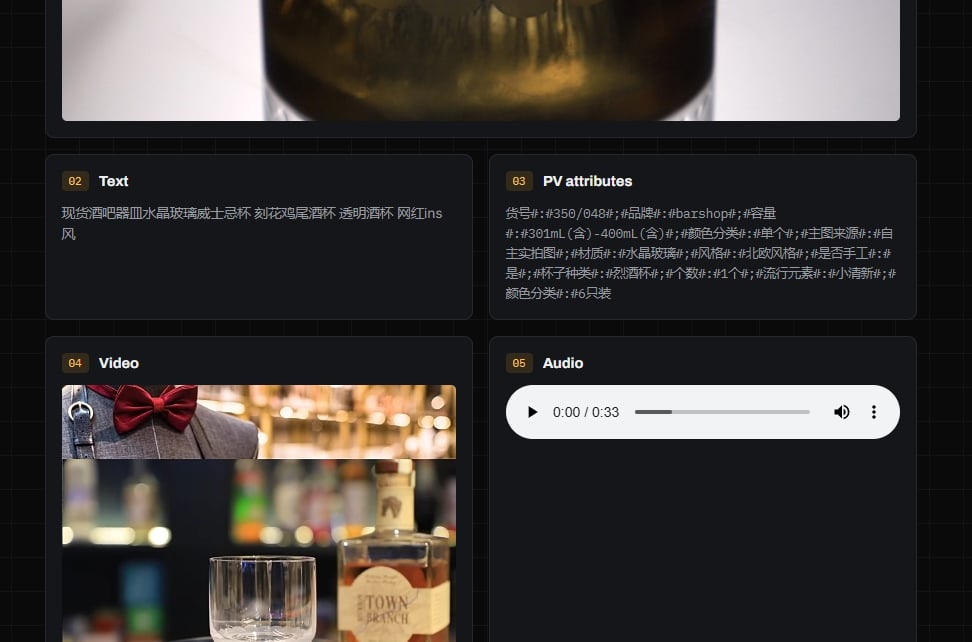
\includegraphics[width=\linewidth]{figure/fe3.jpg}
        \vspace{2pt}

        \small (c) Xem thông tin chi tiết của một sản phẩm từ kết quả retrieval.
    \end{minipage}
    \caption{Ba trạng thái chính của giao diện hệ thống retrieval.}
    \label{fig:frontend-interface}
\end{figure}

\end{document}
